\documentclass[a4paper,11 pt]{article}

%% Language and font encodings
\usepackage[spanish,es-tabla]{babel}
\usepackage[utf8]{inputenc}
\usepackage[T1]{fontenc}
\usepackage{cite}
\usepackage{amsmath, amsthm, amssymb, amsfonts} 
\usepackage[mathscr]{eucal}
\usepackage{ulem} % subrayar, tachar
\usepackage{hyperref} % para el url
\usepackage{multirow, array} % para las tablas
\usepackage{float} % para tablas [H]
\usepackage{graphicx} % graficos
\usepackage{titlesec} %subsubsubsection
\usepackage[usenames]{color} %palabras con color
\usepackage{lscape} % texto horizontal
\usepackage{pdflscape} % hoja horizontal
\usepackage{booktabs} %tabla con puntos
\usepackage{longtable}
\usepackage{url}
\usepackage{listings} 
\usepackage{color}
\usepackage{longtable}
\usepackage{multicol} % documento con doble columna

\titleformat{\paragraph}
{\normalfont\normalsize\bfseries}{\theparagraph}{1em}{}
\titlespacing*{\paragraph}
{0pt}{3.25ex plus 1ex minus .2ex}{1.5ex plus .2ex}

\titleclass{\subsubsubsection}{straight}[\subsection]

\newcounter{subsubsubsection}[subsubsection]
\renewcommand\thesubsubsubsection{\thesubsubsection.\arabic{subsubsubsection}}
\renewcommand\theparagraph{\thesubsubsubsection.\arabic{paragraph}} % optional; useful if paragraphs are to be numbered

\titleformat{\subsubsubsection}
  {\normalfont\normalsize\bfseries}{\thesubsubsubsection}{1em}{}
\titlespacing*{\subsubsubsection}
{0pt}{3.25ex plus 1ex minus .2ex}{1.5ex plus .2ex}

\makeatletter
\renewcommand\paragraph{\@startsection{paragraph}{5}{\z@}%
  {3.25ex \@plus1ex \@minus.2ex}%
  {-1em}%
  {\normalfont\normalsize\bfseries}}
\renewcommand\subparagraph{\@startsection{subparagraph}{6}{\parindent}%
  {3.25ex \@plus1ex \@minus .2ex}%
  {-1em}%
  {\normalfont\normalsize\bfseries}}
\def\toclevel@subsubsubsection{4}
\def\toclevel@paragraph{5}
%\def\toclevel@paragraph{6}
\def\toclevel@subparagraph{6}
\def\l@subsubsubsection{\@dottedtocline{4}{7em}{4em}}
\def\l@paragraph{\@dottedtocline{5}{10em}{5em}}
\def\l@subparagraph{\@dottedtocline{6}{14em}{6em}}
\makeatother

\setcounter{secnumdepth}{4}
\setcounter{tocdepth}{4}

% Break long url
\makeatletter
\g@addto@macro{\UrlBreaks}{\UrlOrds}
\makeatother

\newcolumntype{P}[1]{>{\centering\arraybackslash}p{#1}}
\newcolumntype{M}[1]{>{\centering\arraybackslash}m{#1}}
\newcolumntype{L}[1]{>{\raggedleft\arraybackslash}p{#1}}
\newcolumntype{R}[1]{>{\raggedright\arraybackslash}p{#1}}
  
%counter
\newcounter{mycounter} % create a new counter, called 'mycounter'
% default def'n of '\themycounter' is '\arabic{mycounter}'

%% command to increment 'mycounter' by 1 and to display its value:
\newcommand\showmycounter{\stepcounter{mycounter}\themycounter}

\usepackage{lipsum}
\newcommand\showlips{\stepcounter{mycounter}\lipsum[\value{mycounter}]}

\usepackage[a4paper,top=2cm,bottom=2cm,left=2cm,right=2cm,marginparwidth= 1.5cm]{geometry}
  
\title{\textbf{StoryGraph\\[2.5cm]}}
\normalsize

% Chicos, porfavor incluyan sus nombres en orden alfabetico
\author{\textbf{Documento de Descripción de Arquitectura - Delivery 1}\\[3cm]
        \normalsize{Guiselle Tatiana Zambrano Penagos}\\
        \normalsize{Juan Camilo López Solano}\\
        \normalsize{María José Jara Herrera}\\
        \normalsize{Omar Yecid Orjuela Rodriguez}\\[2.5cm]
        \normalsize{Jeisson Andrés Vergara Vargas}\\[2.5cm]}
\date{}

\begin{document}

\newpage

\begin{figure}
    \centering
    
\includegraphics[width=0.18\textwidth]{images/test.png}
\end{figure}
\maketitle 
\thispagestyle{empty}

\begin{center}
    Universidad Nacional de Colombia\\
    Facultad de Ingeniería\\
    Departamento de Ingeniería de Sistemas e Industrial\\
    Ingeniería de Sistemas\\
    Ingeniería de software basada en la nube\\
    Bogotá, Colombia\\
    2026
\end{center}
\newpage
\tableofcontents % índice de contenido
\thispagestyle{empty}

\newpage


\setcounter{page}{1}
\pagestyle{plain}

\section{Introducción}

\subsection{Equipo}
\subsubsection{Nombre}
1C
\subsubsection{Integrantes}
\begin{multicols}{2}
\begin{itemize}
    \item Omar Yecid Orjuela Rodriguez
    \item Juan Camilo López Solano
    \item María José Jara Herrera
    \item Guiselle Tatiana Zambrano Penagos
\end{itemize}
\end{multicols}
\subsection{Sistema de Software}

\subsubsection{Nombre}
StoryGraph

\subsubsection{Logo}

\begin{figure}[H]
    \centering
    
\includegraphics[width=0.2\textwidth]{images/logo.png}
\end{figure}

\subsubsection{Descripción}

StoryGraph es una plataforma web orientada a la creación, publicación y lectura de historias interactivas no lineales, basada en una estructura narrativa en forma de grafo. El sistema permite a los creadores diseñar relatos en los que cada fragmento narrativo se conecta mediante decisiones que el lector puede seleccionar, generando múltiples caminos y desenlaces posibles.

\subsubsection{Objetivo del proyecto}
Proporcionar un entorno digital que facilite:
\begin{itemize}
    \item La creación estructurada de historias ramificadas.
    \item La exploración interactiva de narrativas dinámicas.
    \item La gestión eficiente de usuarios, contenido y métricas.
    \item La construcción de experiencias personalizadas de lectura.
\end{itemize}

\subsubsection{Valor Diferenciador}
StoryGraph transforma la lectura tradicional en una experiencia interactiva, donde el lector no solo consume contenido, sino que participa activamente en la construcción de la historia. La estructura basada en grafos permite crear narrativas complejas sin necesidad de programación por parte del creador, democratizando la creación de historias interactivas.

\section{Diseño de Arquitectura}
\subsection{Vista de Componentes y Conectores (C\&C)}

\subsubsection{Representación Gráfica}
\begin{figure}[H]
    \centering
    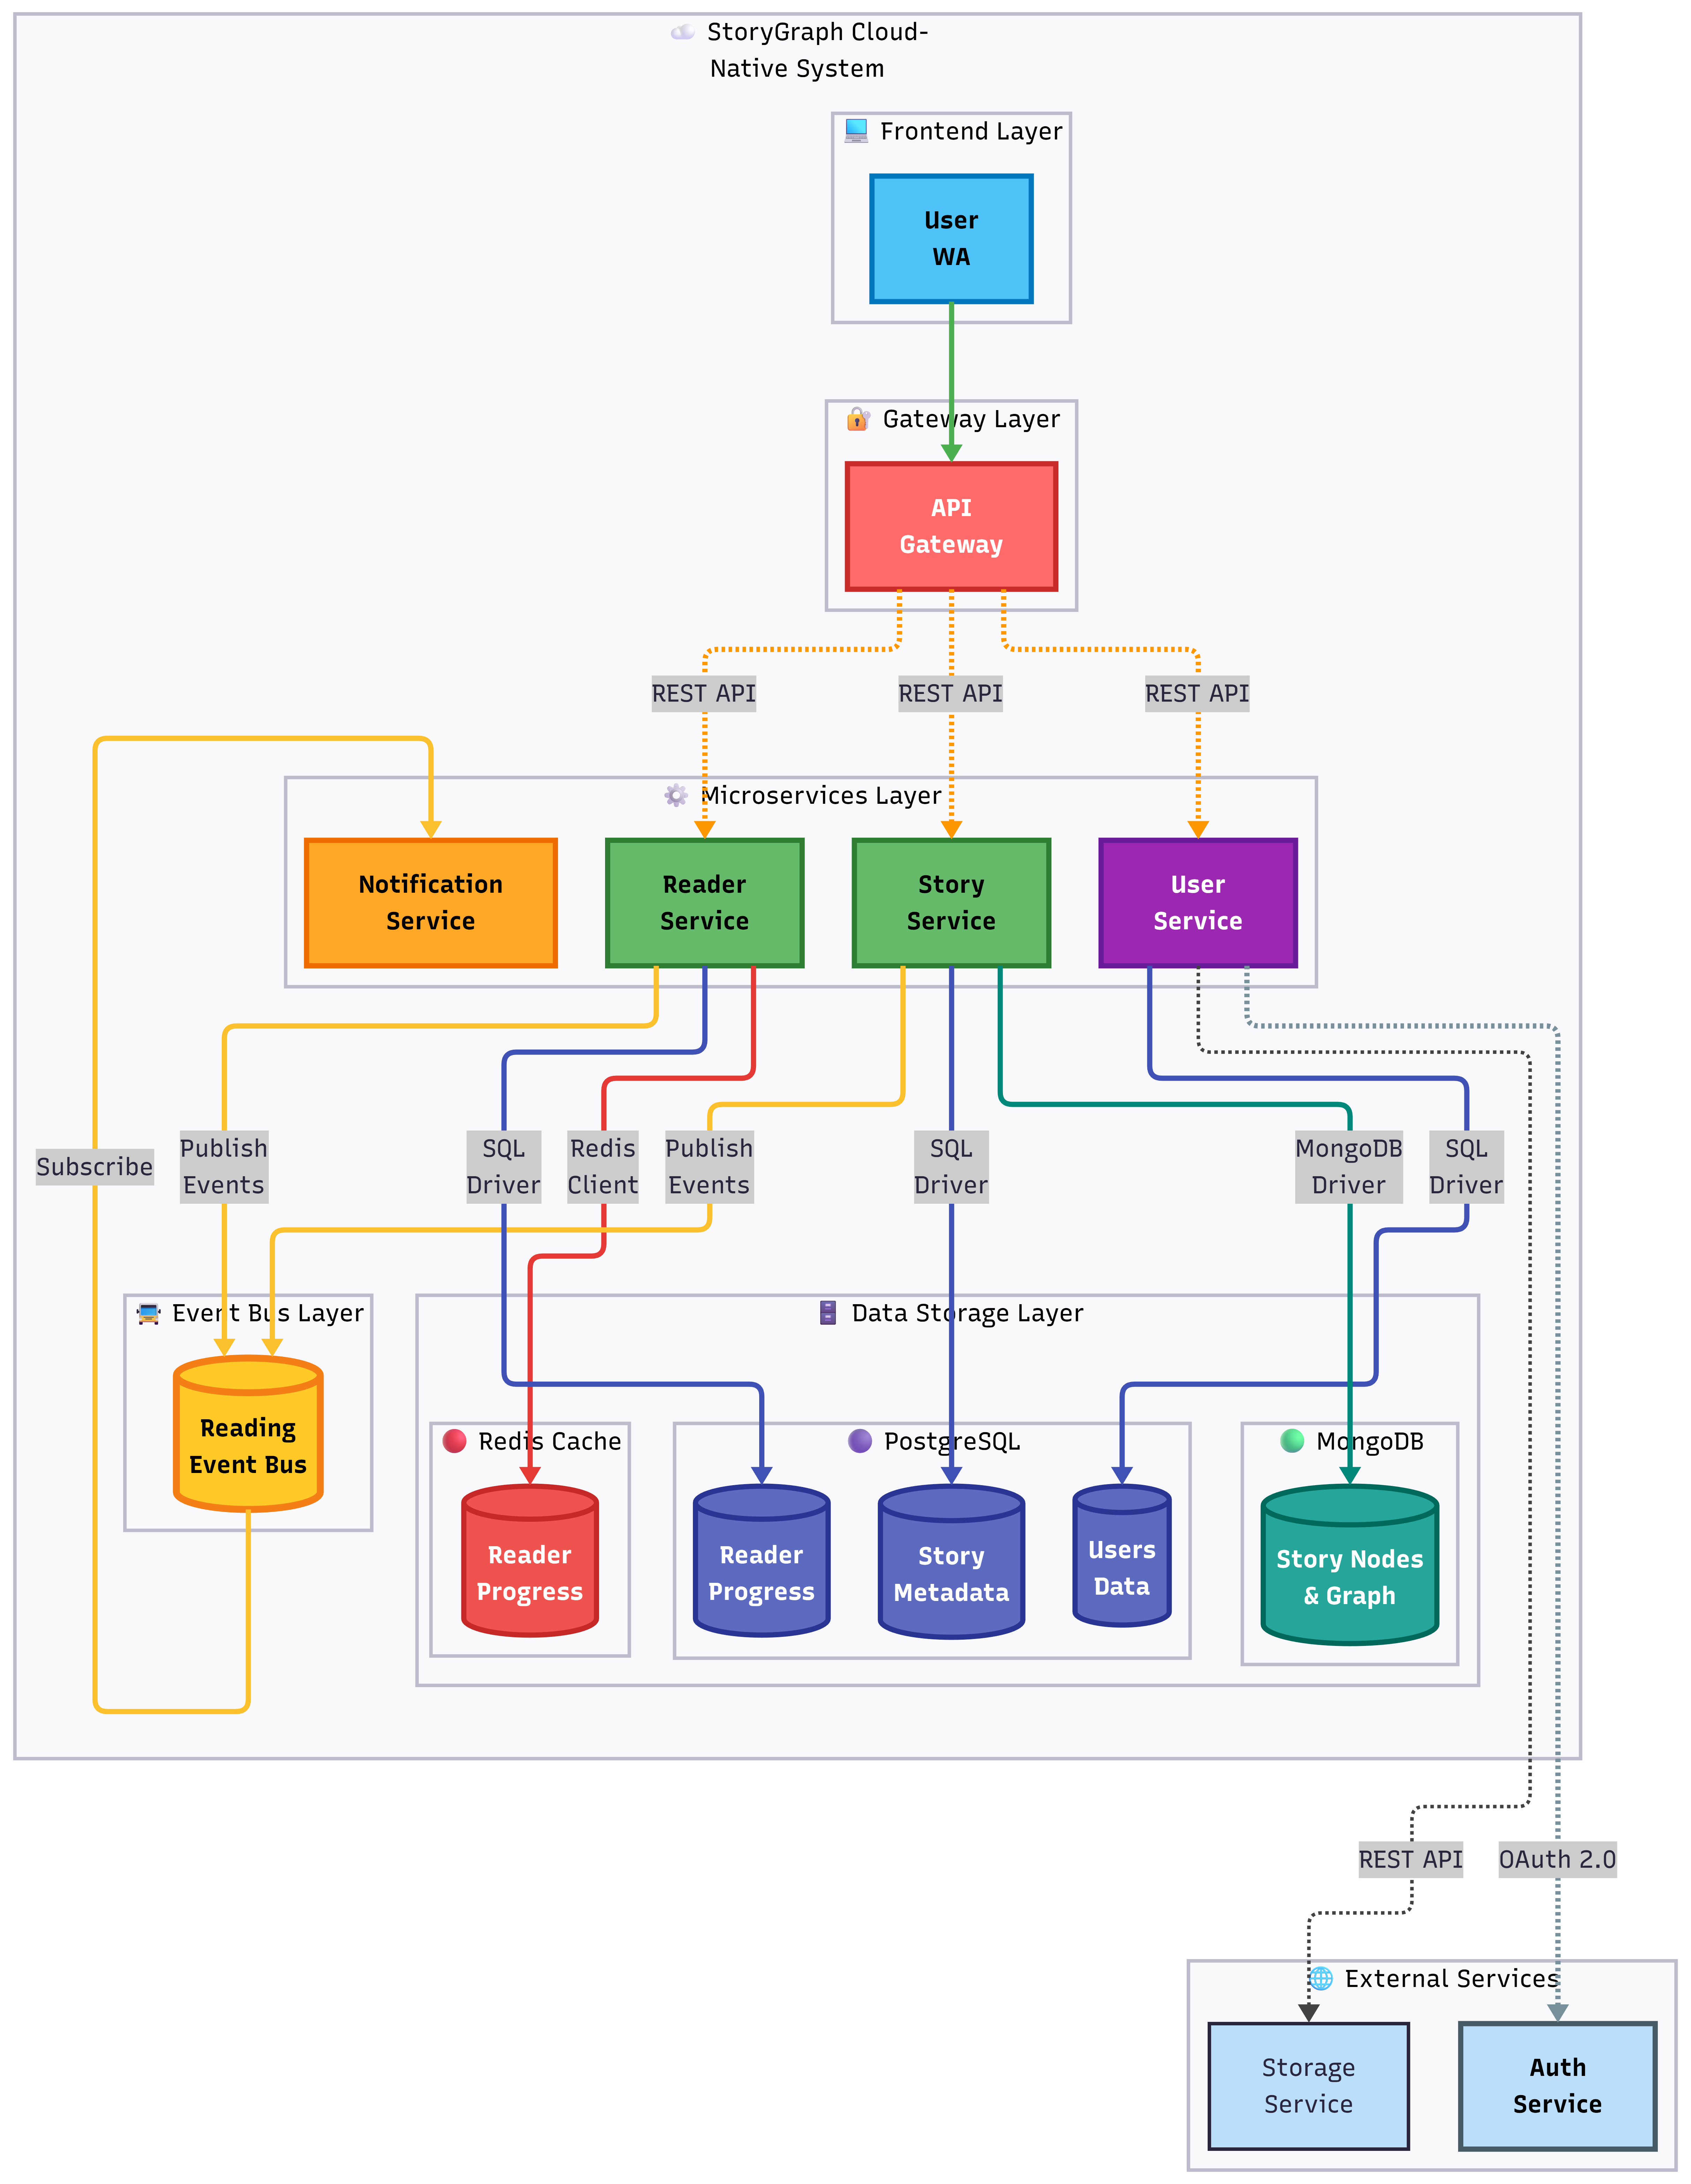
\includegraphics[width=1\textwidth]{images/c&c.png}
\end{figure}
\newpage
\subsubsection{Descripción de la Vista}

Esta vista está compuesta por varios tipos de componentes, a continuación se describirá de manera general dicha clasificación

\begin{table}[H]
    \footnotesize{
    \centering
    \begin{tabular}{|M{3cm}|M{11cm}|}
         \hline
         \textbf{Nombre} & \textbf{Descripción} \\
         \hline
         Interfáz de Programación de Aplicaciones & Componente que contiene acceso a un conjunto de funcionalidades ofrecidas por los microservicios, este es usado como capa de abstracción por el componente del Front-end.\\
         \hline
         Microservicio & Contiene la lógica necesaria para garantizar un conjunto de funcionalidades de alguno de los módulos o sub-módulos del sistema. \\
         \hline
         Base de Datos & Contiene la lógica necesaria para almacenar y obtener de forma adecuada la información procesada por el sistema de software.\\
         \hline
         Aplicación Web & Contiene la estructura visual y lógica para interactuar con el usuario y garantizar el acceso a las funcionalidades del sistema de software a nivel web.\\
         \hline
         Reading Event Bus & Middleware de mensajería asíncrona que desacopla los servicios productores (Story Service, Reading Service) del servicio consumidor Notification service \\
         \hline
         Storage Service & Es un componente externo de infraestructura encargado del almacenamiento y gestión de archivos binarios asociados a los usuarios, tales como fotos de perfil.\\
         \hline
         Authorization Service & Es un componente externo especializado en la gestión de permisos y control de acceso dentro del sistema.\\
         \hline
    \end{tabular}
    \caption{Tipo de sub-componentes que conforman el sistema de software}
    \label{t00}
    }
\end{table}

A continuación se describirá de forma detallada la funcionalidad de cada uno de los componentes y sub-componentes definidos para el sistema:


\begin{itemize}
    \item \textbf{Presentación:} El componente de presentación consta de un componente web que se encargará de gestionar a los usuarios finales (lectores y creadores) y a los administradores.
    \end{itemize}
    
    \begin{table}[H]
    \footnotesize{
        \centering
        \begin{tabular}{|M{2cm}|M{2cm}|M{2cm}|M{8cm}|}
            \hline
             \textbf{Nombre} & \textbf{Lenguaje} & \textbf{Framework} & \textbf{Descripción}\\
             \hline
             User WA & JavaScript & ReactJs & Permite construir interfaces modernas mediante una arquitectura basada en componentes reutilizables que facilitan el mantenimiento y la escalabilidad del proyecto.\\
             \hline 
        \end{tabular}
        \caption{\centering Tecnologías utilizadas los componentes de la capa de presentación}
        \label{t02}}
    \end{table}


\begin{itemize}
    \item \textbf{Logic:} Este componente está conformado por 7 sub-componentes; en la tabla \ref{t06} se especifica la función de cada uno de los sub-componentes y en la tabla \ref{t05} las tecnologías utilizadas en la implementación de los microservicios.

    \begin{table}[H]
    \footnotesize{
        \centering
        \begin{tabular}{|M{2cm}|M{2cm}|M{2cm}|M{8cm}|}
            \hline
             \textbf{Nombre} & \textbf{Lenguaje} & \textbf{Framework} & \textbf{Descripción}\\
             \hline
             User Service & Python & Flask & Ligero y minimalista que permite construir APIs REST de forma rápida, clara y mantenible\\
             \hline
             Story Service & Java & Spring Boot & Es el servicio más complejo en términos de dominio, maneja metadatos, relaciones y lógica de negocio rica. Spring Boot es robusto, tiene soporte nativo para JPA/Hibernate con PostgreSQL, y su tipado estricto reduce errores en modelos de datos complejos.\\
             \hline
             Reader Service & Java & Story Service & Gestiona el progreso de lectura con doble capa de almacenamiento (Redis + PostgreSQL). Spring Boot tiene integraciones maduras con ambos (Spring Data Redis y Spring Data JPA), lo que simplifica la lógica de caché y persistencia.\\
             \hline
             Notification service & JavaScript & Node.js & Es un servicio orientado a eventos, ligero y con alta concurrencia de I/O. El framework tiene un modelo asíncrono que lo hace ideal para consumir colas SQS y despachar notificaciones sin bloquear hilos.\\
             \hline
        \end{tabular}
        \caption{\centering Tecnologías utilizadas para la creación de los sub-componentes de la capa Logic}
        \label{t05}}
    \end{table}
    
    \begin{table}[H]
    \footnotesize{
        \centering
        \begin{tabular}{|M{5cm}|M{9cm}|}
            \hline
            \textbf{Nombre} & \textbf{Descripción} \\
            \hline
             User Service & Microservicio encargado gestionar los datos del usuario como nombre, apellido, display\_name, etc.  \\
             \hline
             Reader Service & Gestión de la interacción del usuario con las historias: progreso de lectura, historias finalizadas, historial de elecciones, navegación nodo a nodo. \\
             \hline
             Story Service & CRUD de historias, gestión de clasificaciones (género, estilo narrativo), gestión de los nodos narrativos que componen cada historia, sus conexiones y validación de la estructura del grafo. \\
             \hline
             Notification Service & Envío de notificaciones a lectores y escritores cuando ocurren eventos relevantes. Ejemplos: cuando un escritor publica una historia, se notifica a los lectores; cuando un lector termina una historia, se notifica al escritor.\\
             \hline
        \end{tabular}
        \caption{\centering Descripción de los micro servicios de la capa Logica.}
        \label{t06}
        }
    \end{table}  
        
    \item \textbf{Data:} Este componente está conformado por 5 sub-componentes de bases de datos, los cuales se encargan de almacenar todos los datos relacionados con los usuarios, las historias, los nodos narrativos y el progreso de lectura de la aplicación. La tabla \ref{t0I} describe las tecnologías utilizadas para la creación de las bases de datos y la tabla \ref{t07} detalla la funcionalidad de cada una.
    
    \begin{table}[H]
        \footnotesize{
        \centering
        \begin{tabular}{|M{5cm}|M{2cm}|M{2cm}|}
            \hline
             \textbf{Nombre} & \textbf{Gestor} & \textbf{Tipo}\\
             \hline
             Reader Progress (Caché)& Redis & NoSQL\\
             \hline
             Reader Progress & PostgreSQL & Relacional\\
             \hline
             Story Metadata & PostgreSQL & Relacional\\
             \hline
             Users Data & PostgreSQL & Relational\\
             \hline
             Story Nodes & MongoDB & NoSQL\\
             \hline
        \end{tabular}
        \caption{\centering Tecnologías utilizadas para la creación de la capa Data.}
        \label{t0I}
        }
    \end{table}
    
    \begin{table}[H]
        \footnotesize{
        \centering
        \begin{tabular}{|M{5cm}|M{9cm}|}
            \hline
             \textbf{Nombre} & \textbf{Descripción} \\
             \hline
             Reader Progress (Caché) & Almacena el estado de lectura activo de cada usuario por historia, optimizado para consultas frecuentes. \\
             \hline
             Reader Progress & Destinado al almacenamiento persistente y consolidado del progreso de los usuarios en todas las historias.\\
             \hline
             Story Metadata &  Su objetivo es gestionar atributos descriptivos, administrativos y clasificatorios de cada historia, que no forman parte directa del contenido narrativo, pero que permiten su organización, búsqueda y control dentro de la plataforma.\\
             \hline
             Story Nodes \& Graph &  Almacena la estructura narrativa completa de cada historia, modelada como un grafo dirigido compuesto por nodos (fragmento narrativo) y conexiones (posibles elecciones para el lector)\\
             \hline
             User Data  & Almacena los datos de perfil del usuario.\\
             \hline
        \end{tabular}
        \caption{\centering Descripción de las bases de datos.}
        \label{t07}
        }
    \end{table}
\end{itemize}

\begin{landscape}
\subsection{Vista de Despliegue}
\subsubsection{Representación Gráfica}

\begin{figure}[H]
    \centering
    
\includegraphics[width=1.15 \textwidth]{images/despliegue.jpg}
\end{figure}
\end{landscape}

\subsubsection{Descripción de elementos}

\subsubsubsection{Cliente — Web Browser}

El punto de entrada al sistema es un navegador web que actúa como dispositivo cliente. Se comunica con la infraestructura de AWS mediante dos protocolos:

\begin{itemize}
    \item \textbf{HTTPS} — hacia las interfaces de usuario (UI Usuario).
    \item \textbf{HTTP} — hacia el API Gateway de AWS para las operaciones de la API.
\end{itemize}

\subsubsubsection{AWS Cloud - Capa Pública}

En la frontera pública de la nube se ubican los siguientes servicios gestionados:

\begin{table}[H]
\centering
\footnotesize
\begin{tabular}{|M{0.2\textwidth}|M{0.7\textwidth}|}
 \hline
    \textbf{Componente} & \textbf{Descripción} \\
    \hline
    UI Usuario & Artefacto estático servido mediante \textbf{CloudFront + S3}. Proporciona la interfaz del lector. \\
     \hline
     Amazon Cognito & Servicio de identidad que implementa \textbf{OAuth 2.0} y emite tokens \textbf{JWT} para autenticación de usuarios. \\
     \hline
     API Gateway & Puerta de enlace de la API (AWS API GW) que aplica \textit{rate limiting} y valida los tokens JWT antes de enrutar las peticiones. \\
     \hline
     Application Load Balancer & Balanceador de carga (ALB) con grupos de destino (\textit{Target Groups}) y verificaciones de salud (\textit{Health Checks}) que distribuye el tráfico HTTP hacia los microservicios internos. \\
     \hline
\end{tabular}
\end{table}

\subsubsubsection{VPC — Subredes Privadas}

Dentro de la VPC privada se alojan los recursos internos del sistema, divididos en dos entornos de ejecución principales: el clúster EKS y la capa de mensajería asíncrona.

\paragraph{3a. EKS Cluster — Microservicios}\mbox{}\\

El clúster de Kubernetes aloja cuatro microservicios desplegados como \textit{pods}:

\begin{table}[H]
\centering
\footnotesize
\begin{tabular}{|M{0.2\textwidth}|M{0.3\textwidth}|M{0.3\textwidth}|}
 \hline
    \textbf{Pod} & \textbf{Imagen / Puerto} & \textbf{Responsabilidad} \\
    \hline
    Reader Service & \texttt{reader-service:latest} / 3001 & Gestión de lectura y progreso del lector. \\
     \hline
     Story Service & \texttt{story-service:latest} / 3002 & Gestión de historias y metadatos narrativos. \\
     \hline
    User Service & \texttt{user-service:latest} / 3003 & Gestión de usuarios. \\
     \hline
    Notification Service & \texttt{notif-service:latest} / 3004 & Envío de notificaciones; actúa como consumidor SQS (AMQP). \\
     \hline
\end{tabular}
\end{table}


\paragraph{3b. Async Messaging Layer — Mensajería Asíncrona}\mbox{}\\

La capa de mensajería desacopla los microservicios productores de eventos de los consumidores. Contiene dos colas \textit{Standard Queue} de \textbf{Amazon SQS}:

\begin{itemize}
    \item \textbf{SQS: story-events} — Recibe eventos relacionados con historias (p.ej., creación, actualización). Los microservicios publican en esta cola mediante AMQP.
    \item \textbf{SQS: reader-events} — Recibe eventos relacionados con el progreso y actividad del lector. El Notification Service consume de esta cola.
\end{itemize}


\paragraph{3c. Amazon S3}\mbox{}\\

Se utiliza como repositorio central de archivos multimedia generados por la plataforma (imágenes de usuario y recursos estáticos de historias), permitiendo que los microservicios almacenen y recuperen contenido de forma desacoplada mediante URLs seguras. Esto evita sobrecargar las bases de datos transaccionales, facilita la entrega eficiente de archivos a los clientes y habilita distribución posterior mediante CDN para mejorar rendimiento y escalabilidad.



\paragraph{3d. Cognito}\mbox{}\\

Servicio administrado de AWS para la autenticación, autorización y gestión de identidades de usuarios. Permite registrar, iniciar sesión y administrar usuarios sin implementar un sistema propio de seguridad.

Soporta estándares abiertos como OAuth 2.0, OpenID Connect y SAML, generando y validando tokens JWT (ID Token, Access Token y Refresh Token) para proteger APIs y aplicaciones web/móviles.

\subsubsubsection{Capa de Almacenamiento de Datos (Data Stores)}

Los datos persistentes se distribuyen entre varios servicios de almacenamiento gestionados por AWS:

\begin{table}[H]
\centering
\footnotesize
\begin{tabular}{|M{0.2\textwidth}|M{0.3\textwidth}|M{0.3\textwidth}|}
 \hline
    \textbf{Artefacto} & \textbf{Tecnología} & \textbf{Descripción} \\
    \hline
    Reader Progress (caché) & Amazon ElastiCache Redis & Almacenamiento en memoria del progreso de lectura con acceso rápido (TCP 6379). \\
     \hline
     Reader Progress (persistente) & Amazon RDS PostgreSQL & Base de datos relacional para persistencia del progreso (TCP 5432). \\
     \hline
    Story Metadata & Amazon RDS PostgreSQL & Almacena los metadatos de las historias (TCP 5432). \\
     \hline
    Users & Amazon RDS PostgreSQL & Datos de usuarios (TCP 5432). \\
     \hline
     Story Nodes \& Graph & MongoDB & Base de datos de grafos para modelar nodos y relaciones entre historias. \\
     \hline
\end{tabular}
\end{table}


\section{Diseño detallado}
\subsection{Modelo de datos}

\begin{enumerate}
    \item \textbf{User Service: user\_profiles}\newline
        \textbf{Tecnología}: PostgreSQL\newline
        \textbf{Descripción}: Almacena el perfil público de cada usuario: nombre, apellido, nombre de pantalla (display\_name), biografía y URL de foto de perfil. Vinculado por FK lógica al user\_id del Auth Service.
    \begin{figure}[H]
        \centering
        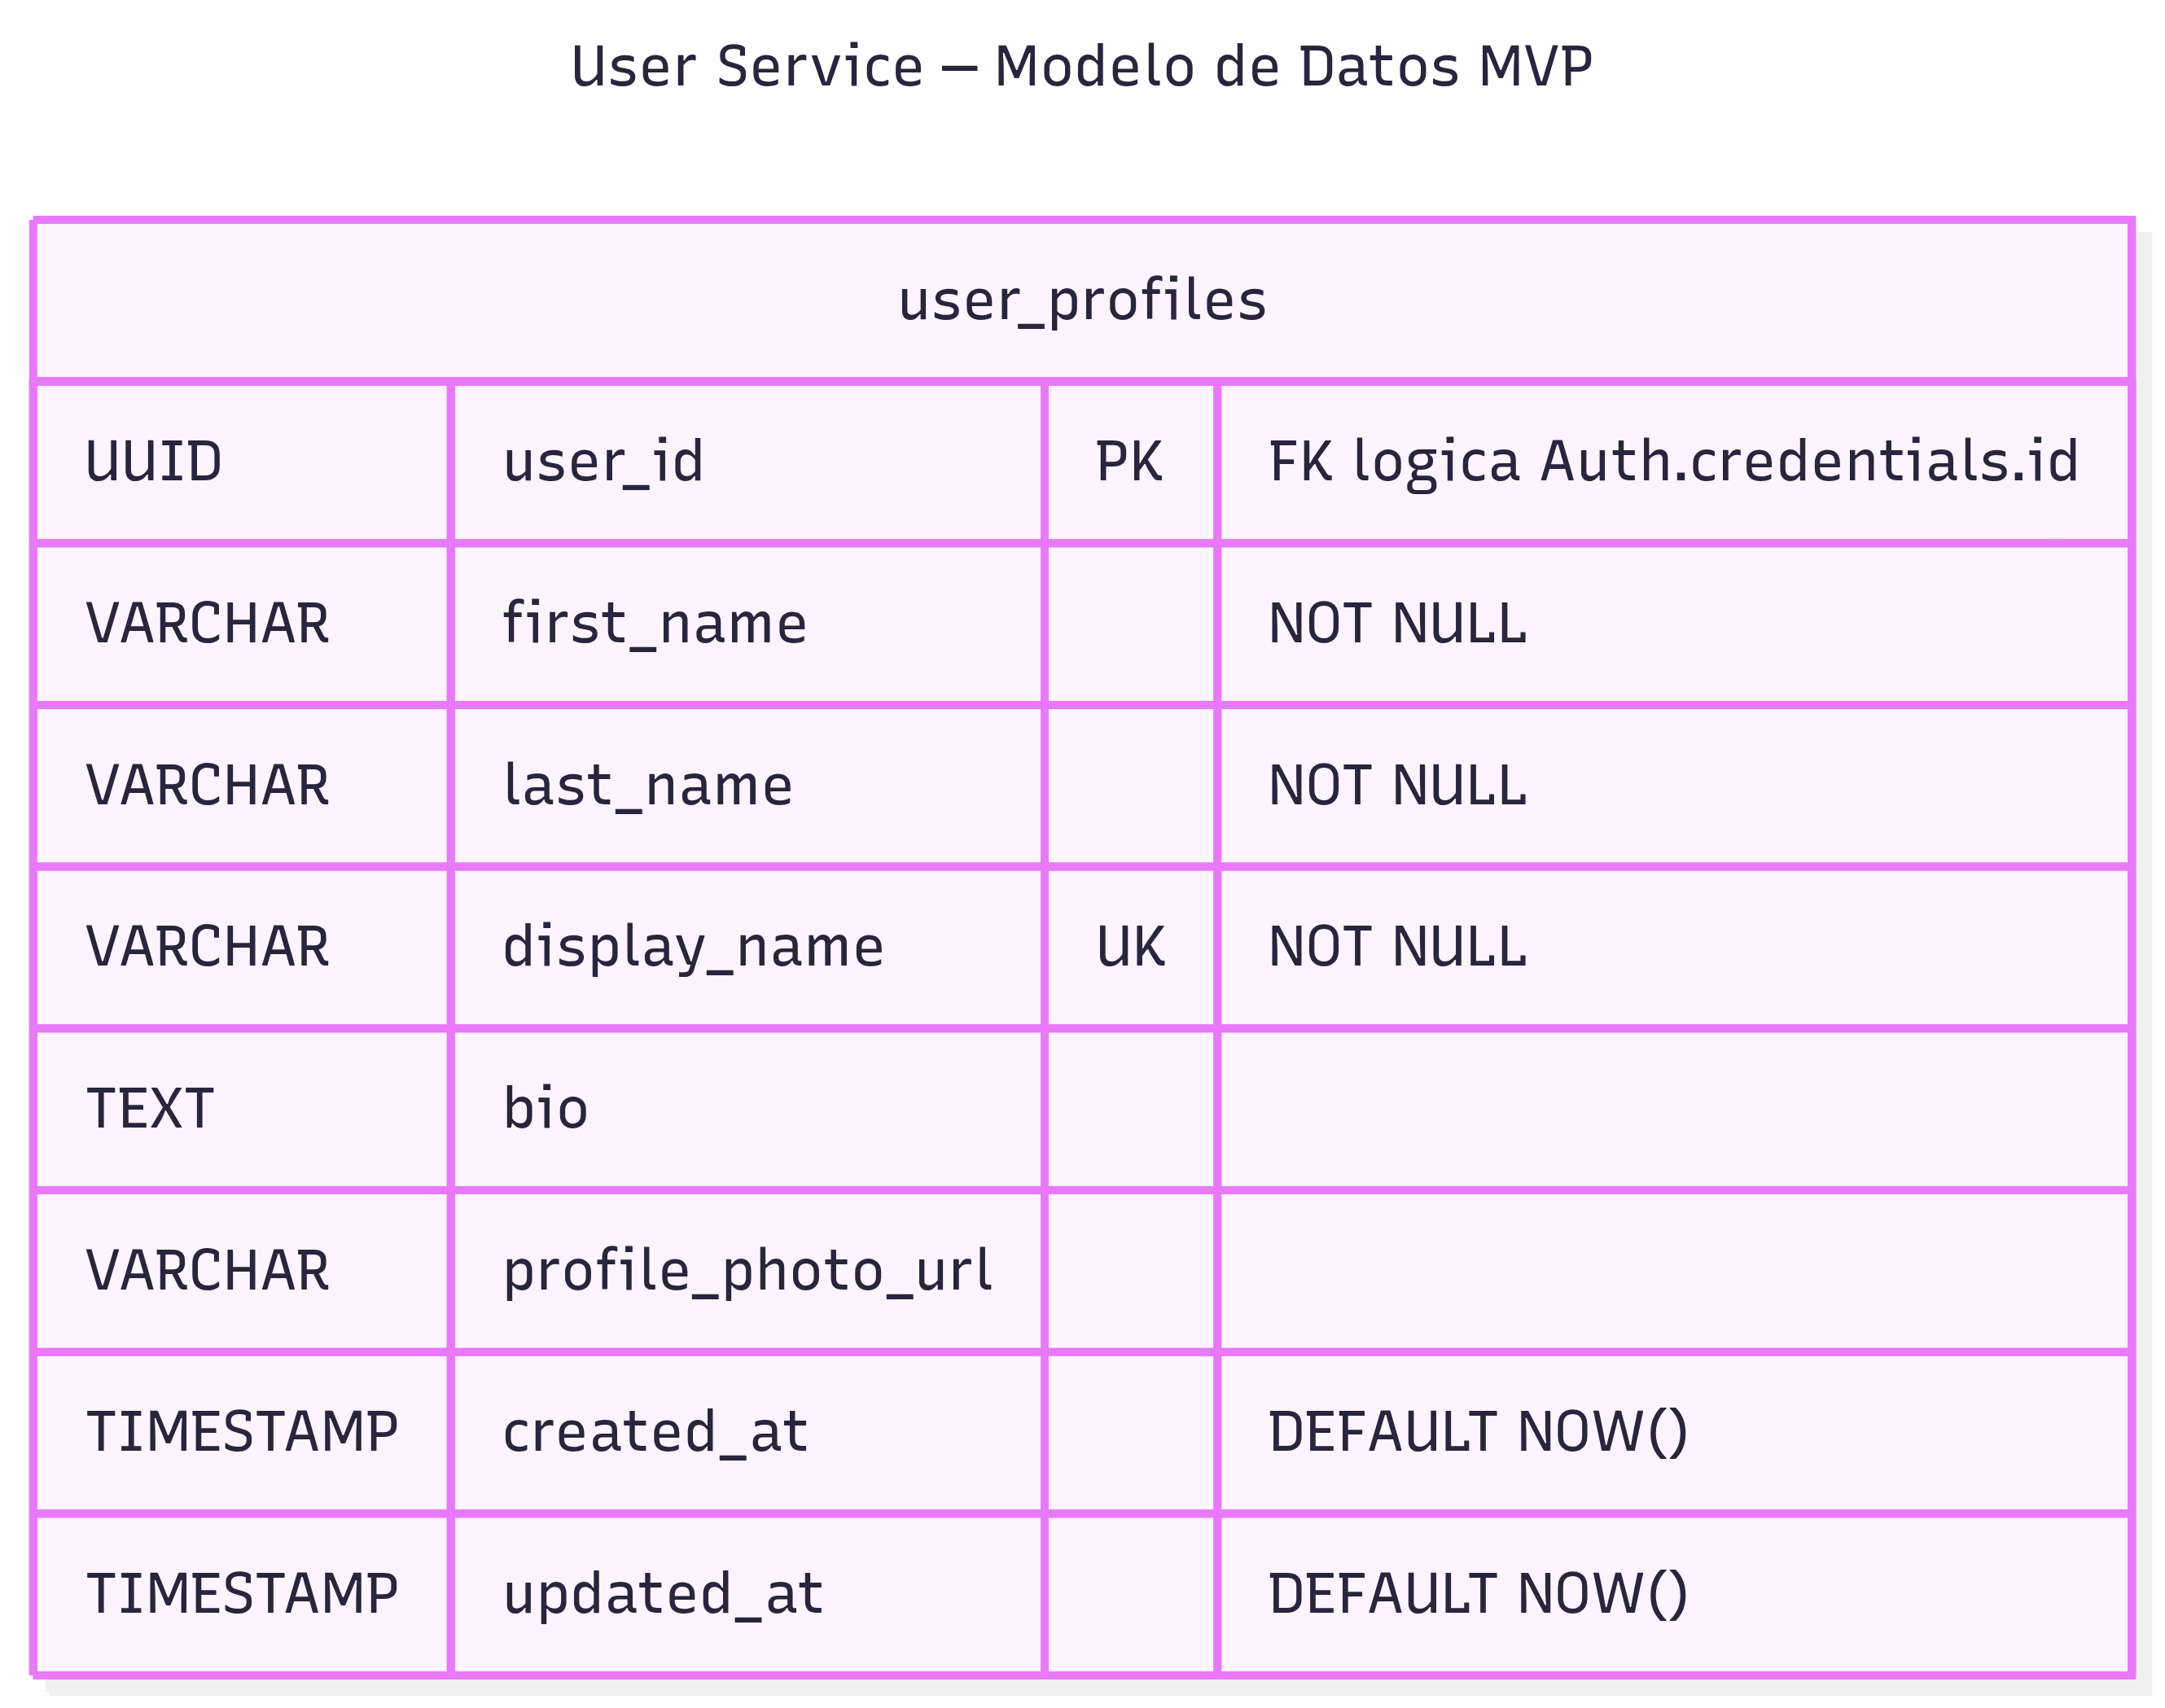
\includegraphics[width=0.5\textwidth]{images/user-data-model.png}
    \end{figure}

    \item \textbf{Story Service: stories y nodes}\newline
        \textbf{Tecnología}: MongoDB\newline
        \textbf{Descripción}: Almacena el grafo narrativo: la colección stories guarda la configuración de cada historia (nodo raíz) y la colección nodes guarda cada nodo narrativo con su contenido, opciones de elección (choices) y si es nodo inicial o final.
    \begin{figure}[H]
        \centering
        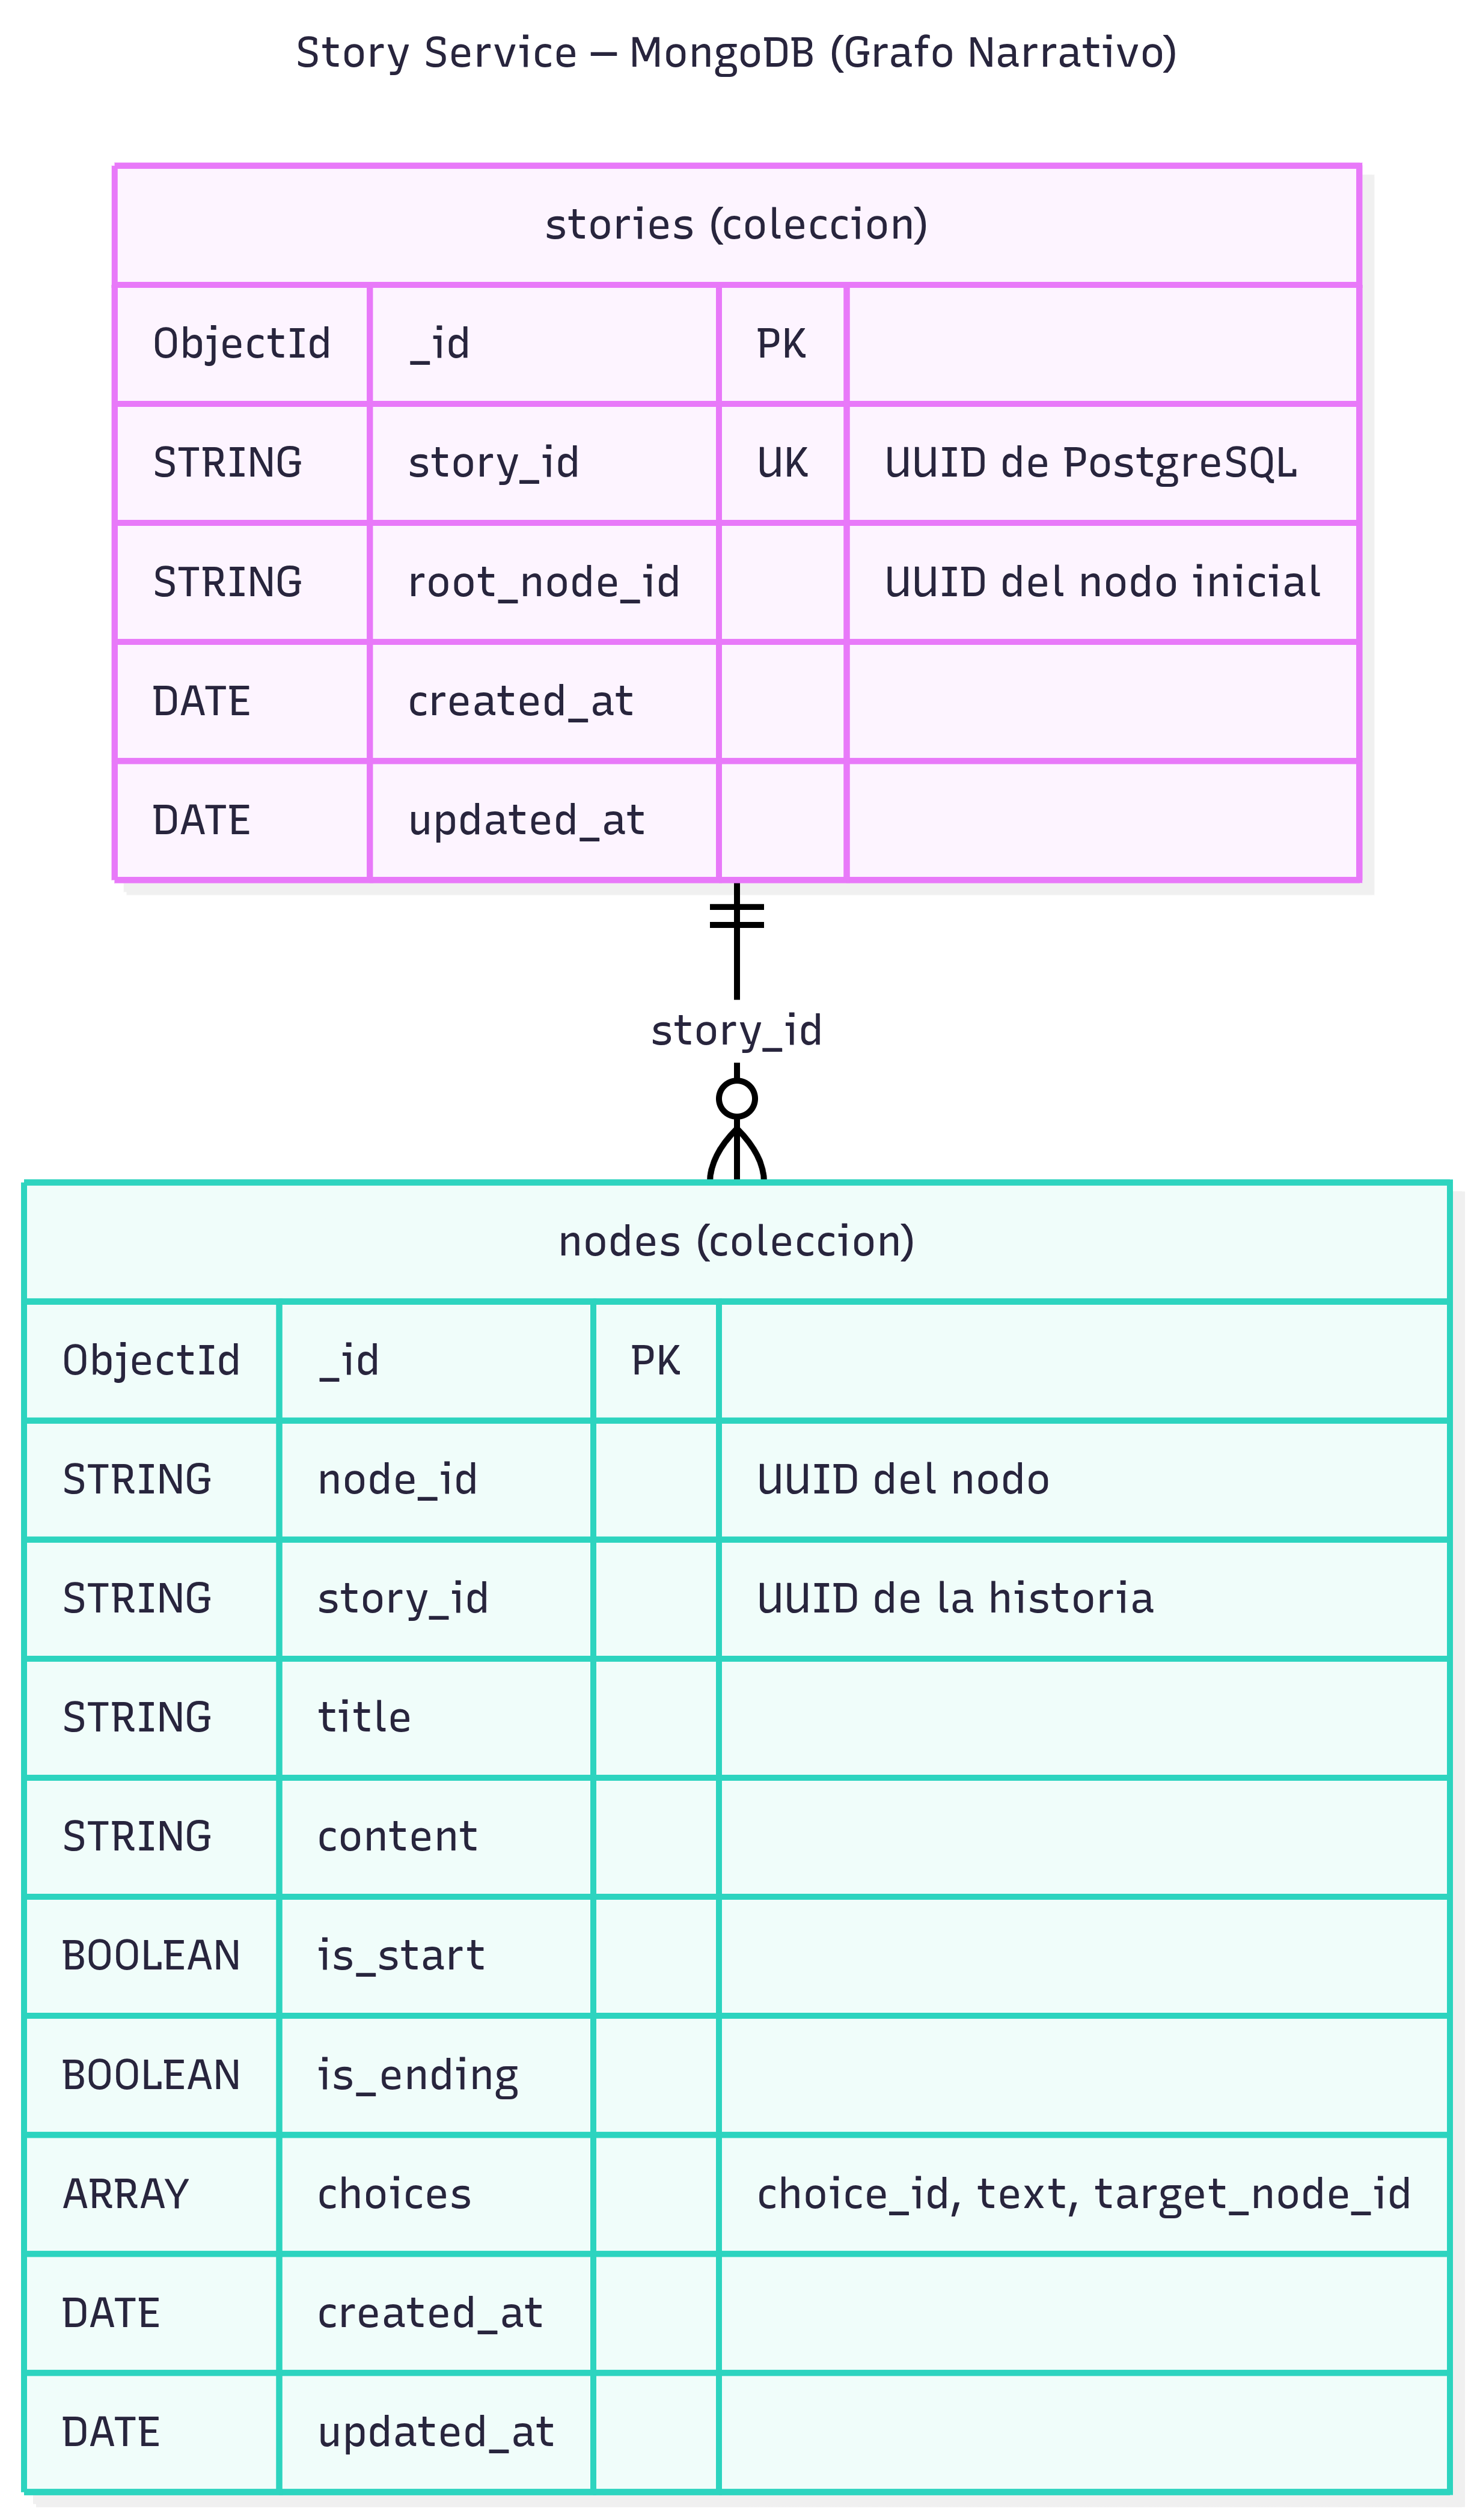
\includegraphics[width=0.5\textwidth]{images/story-data-model.png}
    \end{figure}

    \newpage
    \item \textbf{Story Service: stories y nodes}\newline
        \textbf{Tecnología}: PostgreSQL\newline
        \textbf{Descripción}: Almacena los metadatos de las historias (título, sinopsis, estado, versión, conteo de nodos) y el catálogo de géneros literarios. Funciona como registro maestro para las historias del sistema.
    \begin{figure}[H]
        \centering
        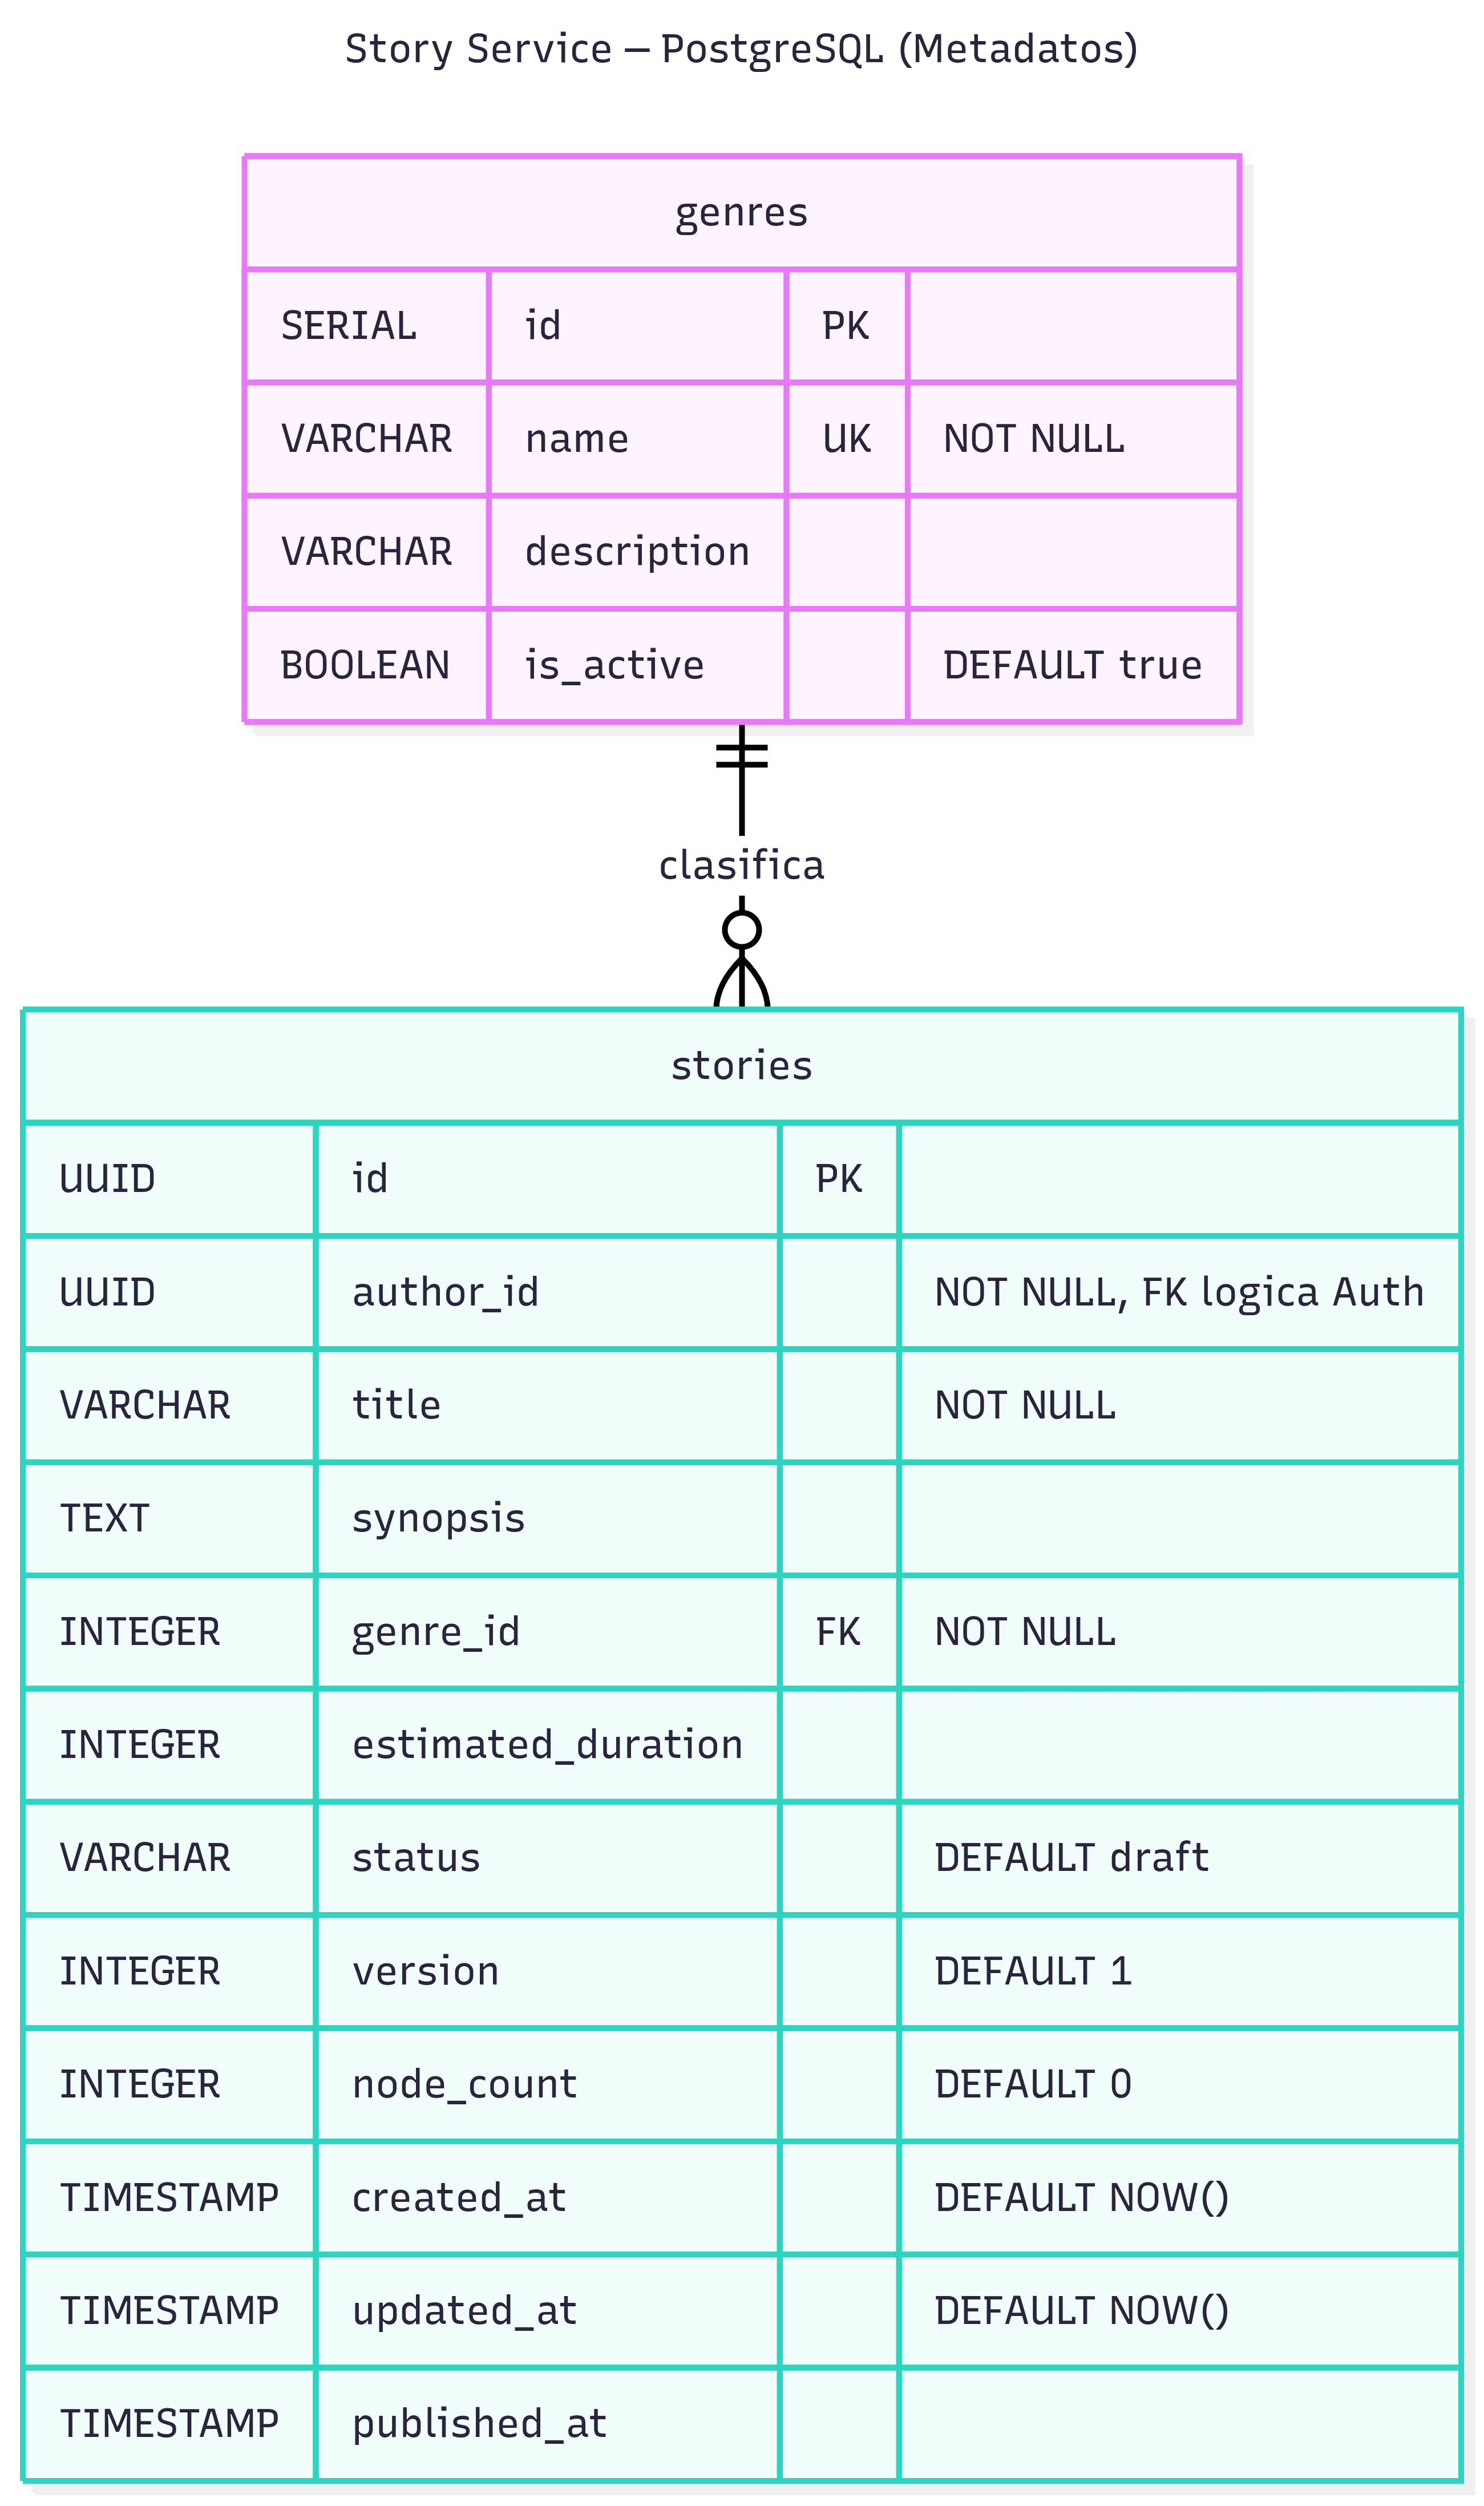
\includegraphics[width=0.5\textwidth]{images/story-data-model-metadata.png}
    \end{figure}

    \item \textbf{Reading Service: reading\_sessions y choice\_history}\newline
        \textbf{Tecnología}: PostgreSQL\newline
        \textbf{Descripción}: Almacena las sesiones de lectura (qué usuario está leyendo qué historia, en qué nodo va, estado de la sesión) y el historial secuencial de elecciones tomadas por el lector en cada sesión.
    \begin{figure}[H]
        \centering
        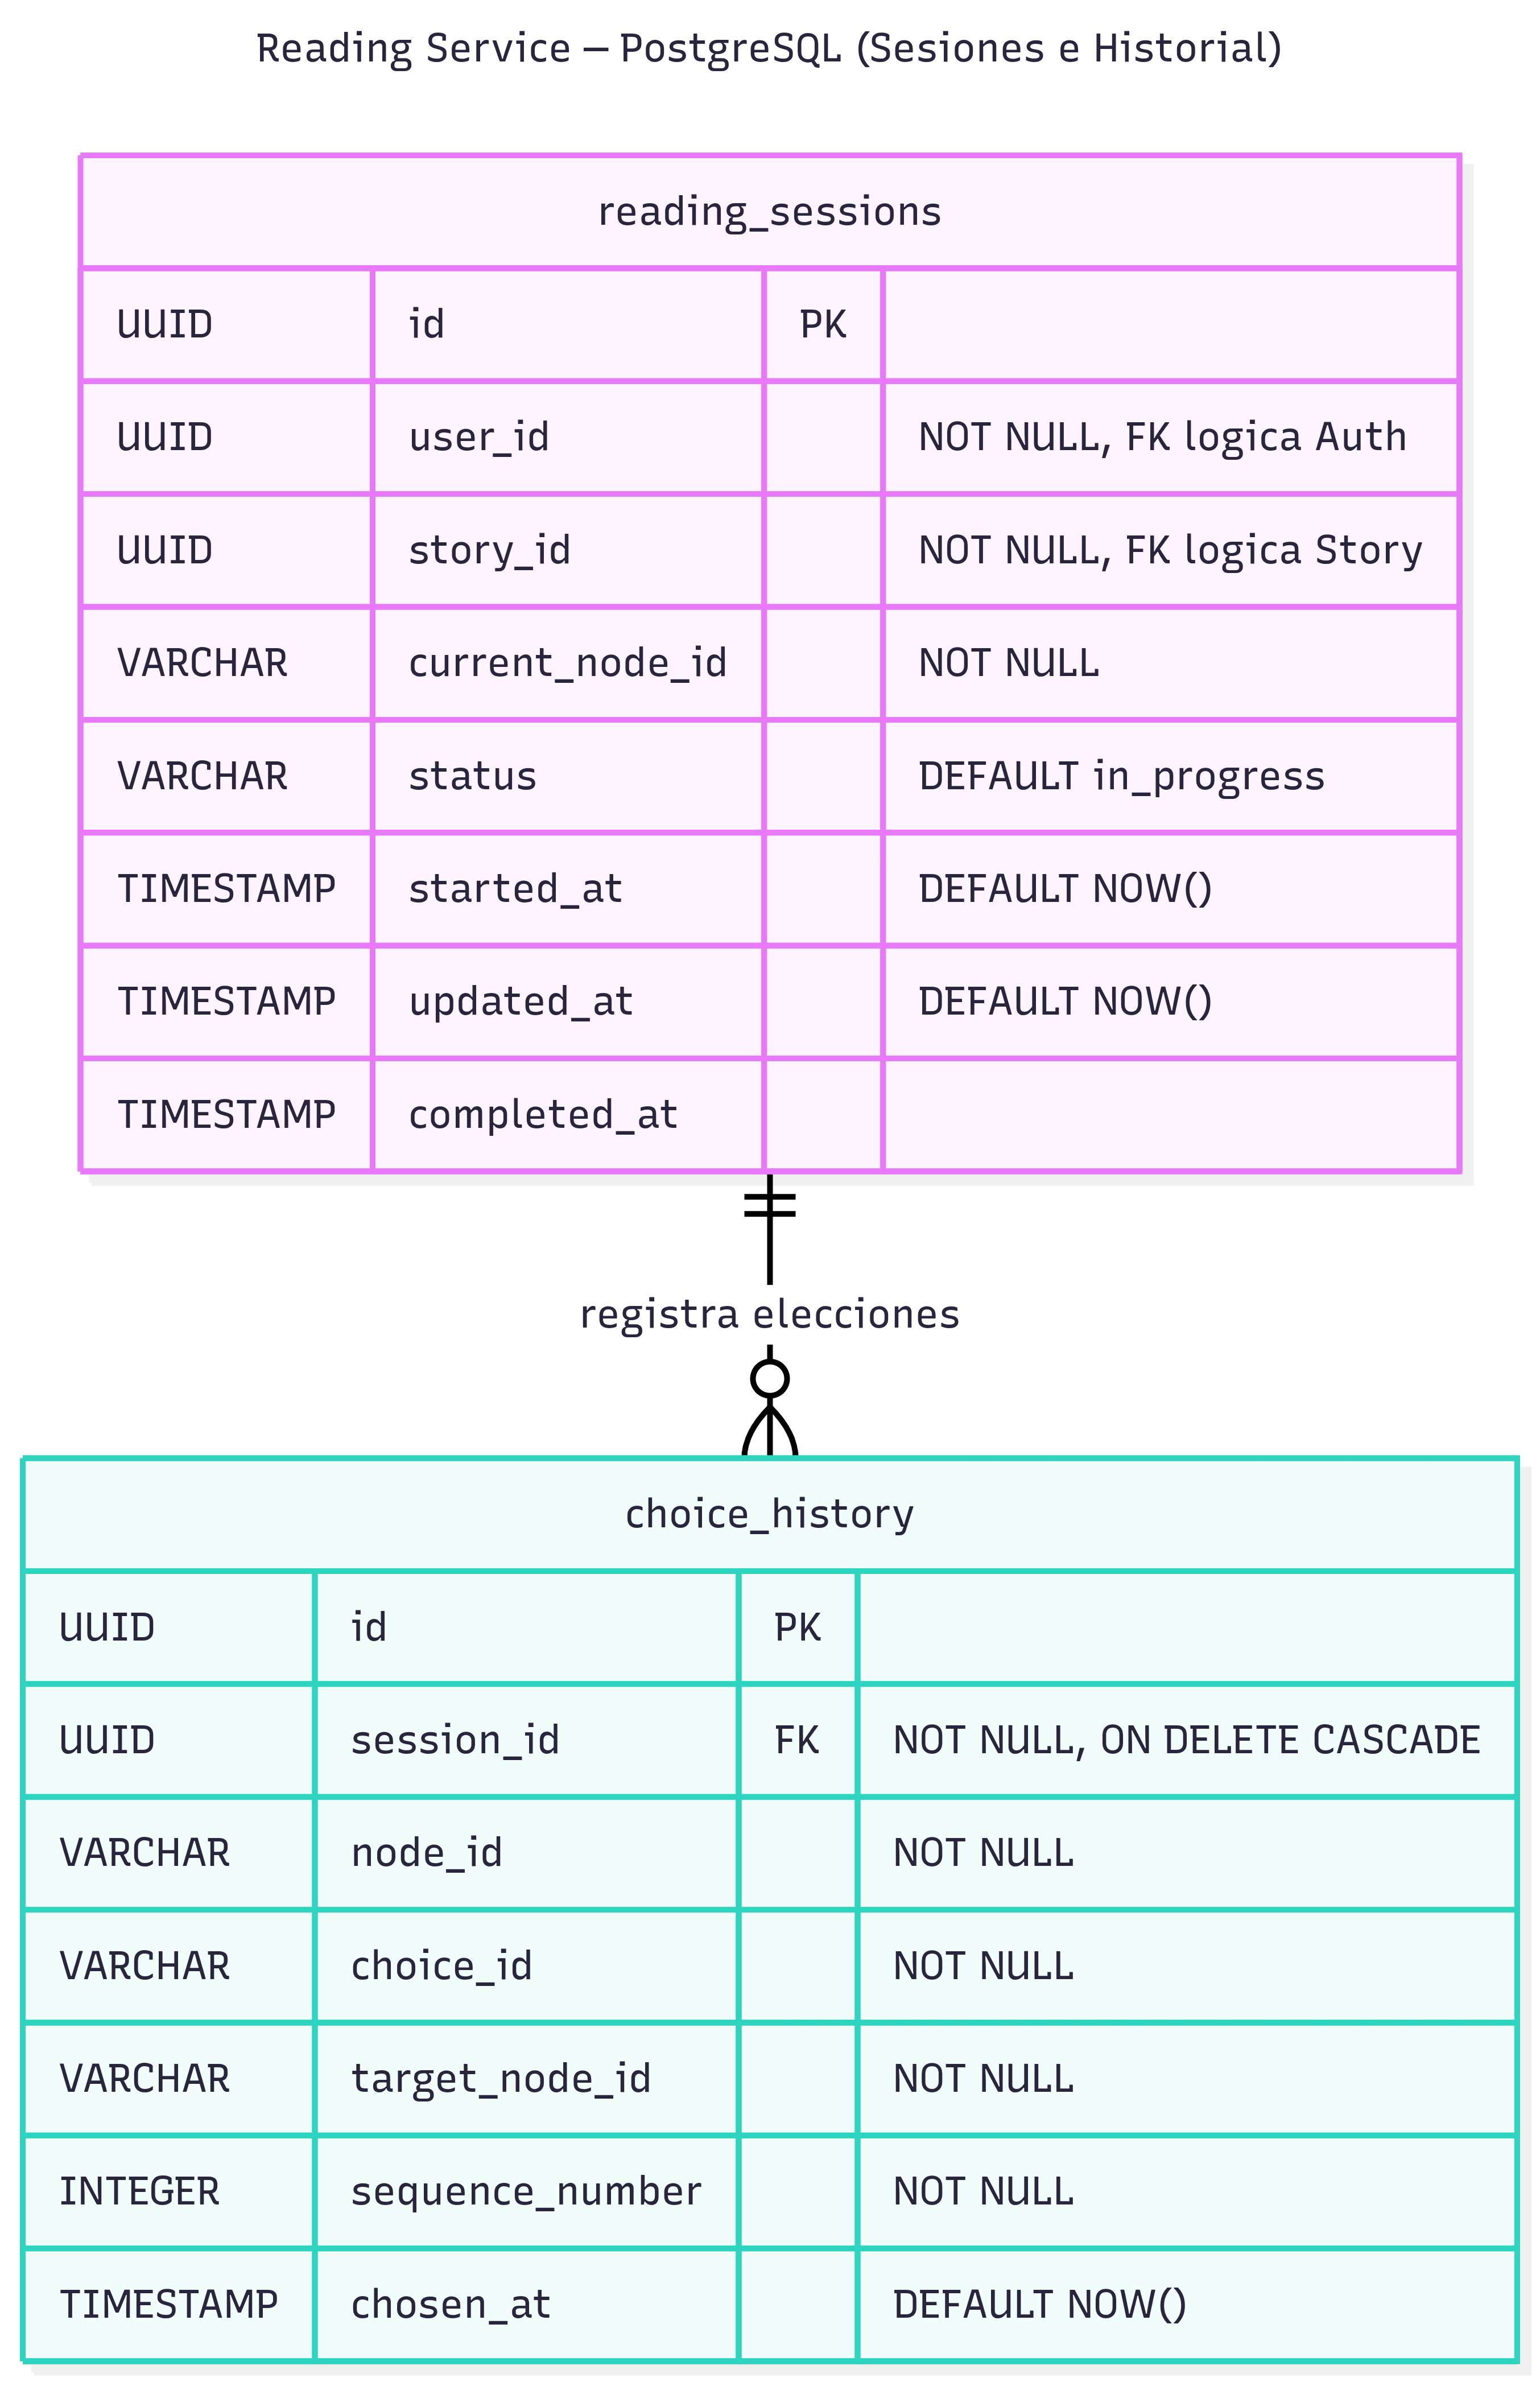
\includegraphics[width=0.5\textwidth]{images/reading-data-model.png}
    \end{figure}

    \item \textbf{Reading Service: cache}\newline
        \textbf{Tecnología}: Redis\newline
        \textbf{Descripción}: Cache de lectura con dos patrones de claves: node:{story\_id}:{node\_id} cachea el contenido completo del nodo de MongoDB (TTL 1h), y progress:{user\_id}:{story\_id} cachea el progreso actual del lector para acceso rápido (TTL 30min).
    \begin{figure}[H]
        \centering
        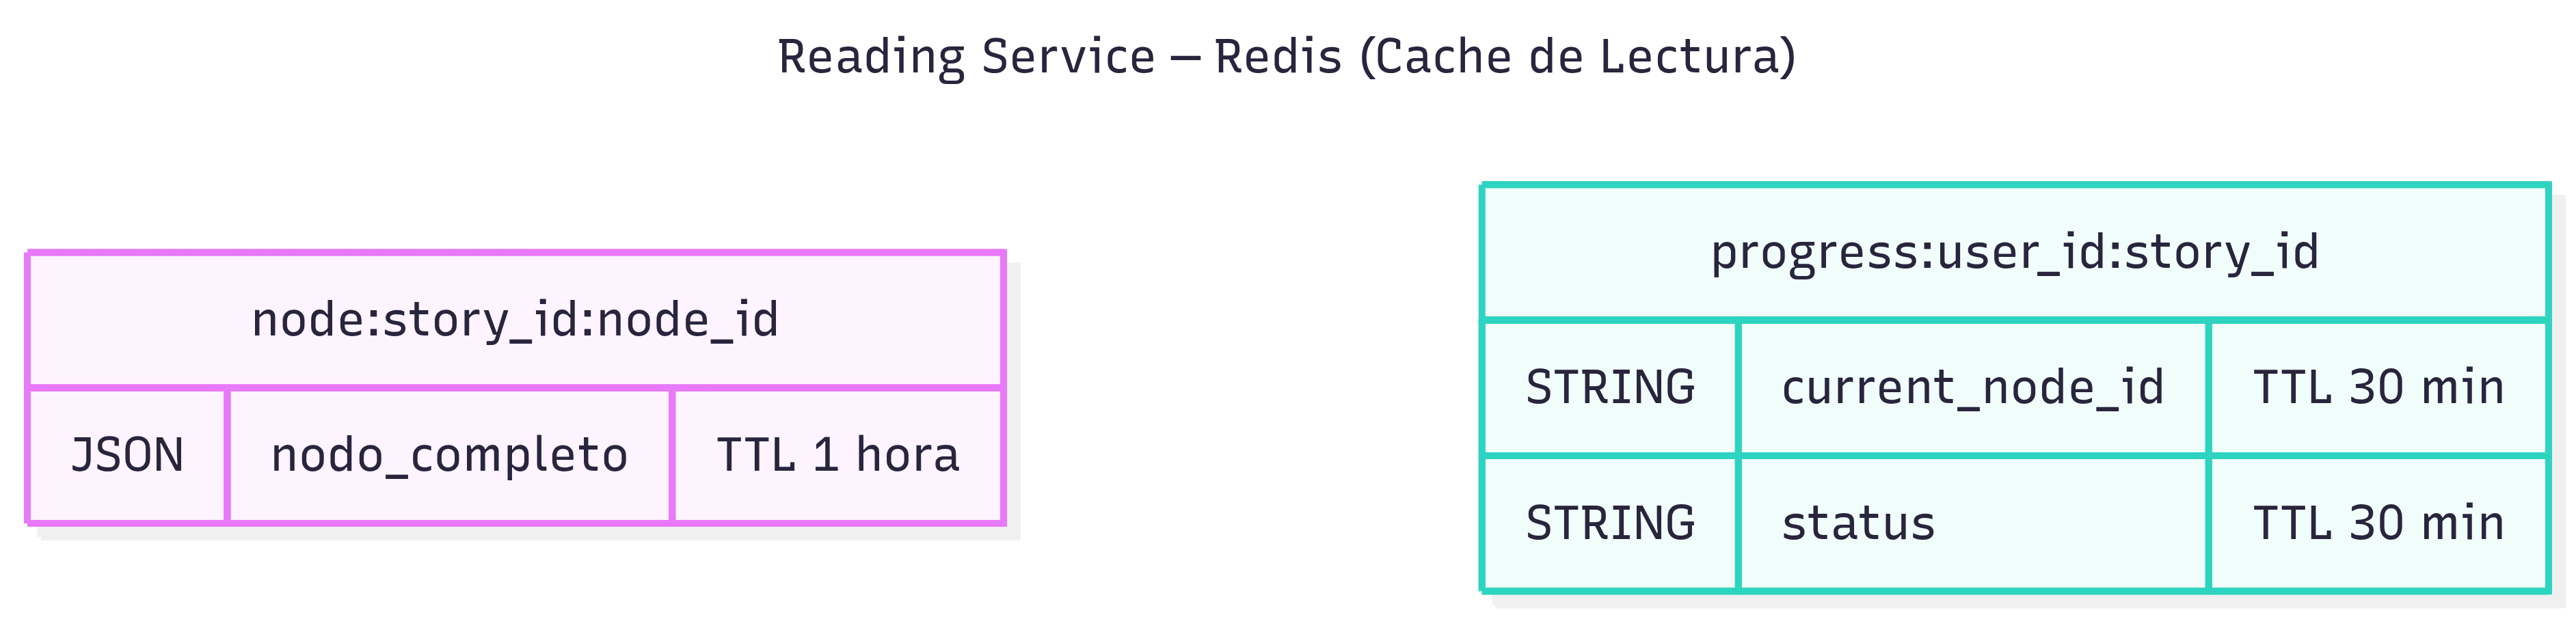
\includegraphics[width=0.8\textwidth]{images/reading-redis-model.png}
    \end{figure}
    
\end{enumerate}

\subsection{Specificación del API}

\subsubsection{Tabla de ruteo}

\begin{table}[H]
\centering
\footnotesize
\begin{tabular}{|M{0.3\textwidth}|M{0.6\textwidth}|}
    \hline
    \textbf{Ruta} & \textbf{Microservicio de destino} \\
    \hline
     /auth/* & Auth service  \\
     \hline
     /users/* & User Service \\
     \hline
     /stories/* & Story Service \\
     \hline
     /read/* & Reading Service\\
     \hline
\end{tabular}
\label{t10}
\end{table}

\subsubsection{Microservicios}
\begin{itemize}
    \item \textbf{Auth Service}
    \begin{table}[H]
        \footnotesize{
        \centering
        \begin{tabular}{|M{0.1\textwidth}|M{0.2\textwidth}|M{0.5\textwidth}|}
            \hline
            \textbf{Tipo} &\textbf{Endpoint} & \textbf{Descripción} \\
            \hline
             POST & /auth/register & Registro de nuevo usuario.  \\
             \hline
             POST & /auth/login & Inicio de sesión, retorna access + refresh token. \\
             \hline
             POST & /auth/refresh & Renovar access token. \\
             \hline
             POST & /auth/logout & Invalidar tokens.\\
             \hline
             GET & /auth/verify & Verificar validez de un token\\
             \hline
        \end{tabular}
        \label{t11}
        }
    \end{table}
    \item \textbf{User Service}
    \begin{table}[H]
        \footnotesize{
        \centering
        \begin{tabular}{|M{0.1\textwidth}|M{0.2\textwidth}|M{0.5\textwidth}|}
            \hline
            \textbf{Tipo} &\textbf{Endpoint} & \textbf{Descripción} \\
            \hline
             GET & /users/:id & Obtener perfil de usuario.  \\
             \hline
             PUT & /users/:id & Actualizar datos de perfil. \\
             \hline
             DELETE & /users/:id & Eliminar cuenta de usuario. \\
             \hline
             GET & /users & Listar usuarios (admin).\\
             \hline
        \end{tabular}
        \label{t12}
        }
    \end{table}
    \item \textbf{Story Service}
    \begin{table}[H]
        \footnotesize{
        \centering
        \begin{tabular}{|M{0.1\textwidth}|M{0.3\textwidth}|M{0.4\textwidth}|}
            \hline
            \textbf{Tipo} &\textbf{Endpoint} & \textbf{Descripción} \\
            \hline
             POST & /stories & Crear historia.  \\
             \hline
             GET &/stories/:id & Obtener metadatos de una historia. \\
             \hline
             PUT & /stories/:id & Actualizar metadatos. \\
             \hline
             POST & /stories/:id/publish & Publicar historia.\\
             \hline
             DELETE &/stories/:id & Eliminar historia.\\
             \hline
             GET &/stories/:id/nodes & Obtener todos los nodos de una historia.\\
             \hline
             POST &/stories/:id/nodes & Crear nodo\\
             \hline
             PUT & /stories/:id/nodes/:nodeId & Editar nodo.\\
             \hline
             DELETE & /stories/:id/nodes/:nodeId & Eliminar nodo.\\
             \hline
             POST & /stories/:id/nodes/:nodeId/choices & Agregar elección/conexión a otro nodo.\\
             \hline
             GET & /stories/:id/graph & Obtener grafo completo (para visualizador).\\
             \hline
             GET & /stories/genres & Listar géneros disponibles.\\
             \hline
        \end{tabular}
        \label{t13}
        }
    \end{table}

    \begin{table}[H]
        \footnotesize{
        \centering
        \begin{tabular}{|M{0.4\textwidth}|M{0.5\textwidth}|}
            \hline
            \textbf{Evento que emite} & \textbf{Descripción} \\
            \hline
             story.created & Historia creada.  \\
             \hline
             story.published & Historia publicada.  \\
             \hline
        \end{tabular}
        \label{t13}
        }
    \end{table}
    
    \item \textbf{Reading Service}
    \begin{table}[H]
        \footnotesize{
        \centering
        \begin{tabular}{|M{0.1\textwidth}|M{0.3\textwidth}|M{0.4\textwidth}|}
            \hline
            \textbf{Tipo} &\textbf{Endpoint} & \textbf{Descripción} \\
            \hline
             GET & /read/:storyId/start & Iniciar lectura, obtener nodo inicial.  \\
             \hline
             GET & /read/:storyId/node/:nodeId & Obtener nodo y sus opciones. \\
             \hline
             POST & /read/:storyId/choose & Registrar elección y avanzar al siguiente nodo. \\
             \hline
             GET & /read/:storyId/progress & Obtener progreso guardado.\\
             \hline
             GET & /read/:storyId/history & Historial de elecciones del lector.\\
             \hline
             GET & /read/my-stories & Listar historias en progreso y finalizadas del usuario.\\
             \hline
             DELETE & /read/:storyId/progress & Reiniciar progreso de una historia.\\
             \hline
        \end{tabular}
        \label{t13}
        }
    \end{table}

    \begin{table}[H]
        \footnotesize{
        \centering
        \begin{tabular}{|M{0.4\textwidth}|M{0.5\textwidth}|}
            \hline
            \textbf{Evento que emite} & \textbf{Descripción} \\
            \hline
             reader.story\_started & El lector inicia una historia..  \\
             \hline
             reader.story\_completed & El lector llega a un nodo final  \\
             \hline
        \end{tabular}
        \label{t13}
        }
    \end{table} 
\end{itemize}

\subsection{Flujos Funcionales (User - GUI)}

\subsubsection{Creación una historia}
El creador inicia una nueva historia desde la UI, que se registra en el Story Service en estado draft. Luego, mediante un editor visual de grafos, construye la narrativa en tres pasos: primero crea el nodo raíz (punto de inicio), después agrega nodos adicionales (fragmentos narrativos, algunos marcados como finales), y finalmente conecta los nodos mediante choices (las opciones que verá el lector). Una vez armado el grafo, el creador puede validar la estructura para verificar que exista un nodo raíz, al menos un nodo final y que todos los nodos sean alcanzables.
\begin{figure}[H]
    \centering
    \includegraphics[width=1\textwidth]{images/flujo-story-creation.png}
\end{figure}



\subsubsection{Lectura de una historia}
El lector selecciona una historia y el Reading Service crea una sesión de lectura, solicitando el nodo raíz al Story Service. A partir de ahí comienza un bucle interactivo: el lector lee el texto narrativo, elige una opción, el Reading Service registra cada elección en el historial y obtiene el siguiente nodo. Cuando el lector alcanza un nodo final, la sesión se marca como completada, se emite reader.story\_completed y el Notification Service notifica al autor de que alguien terminó su historia.

\begin{figure}[H]
    \centering
    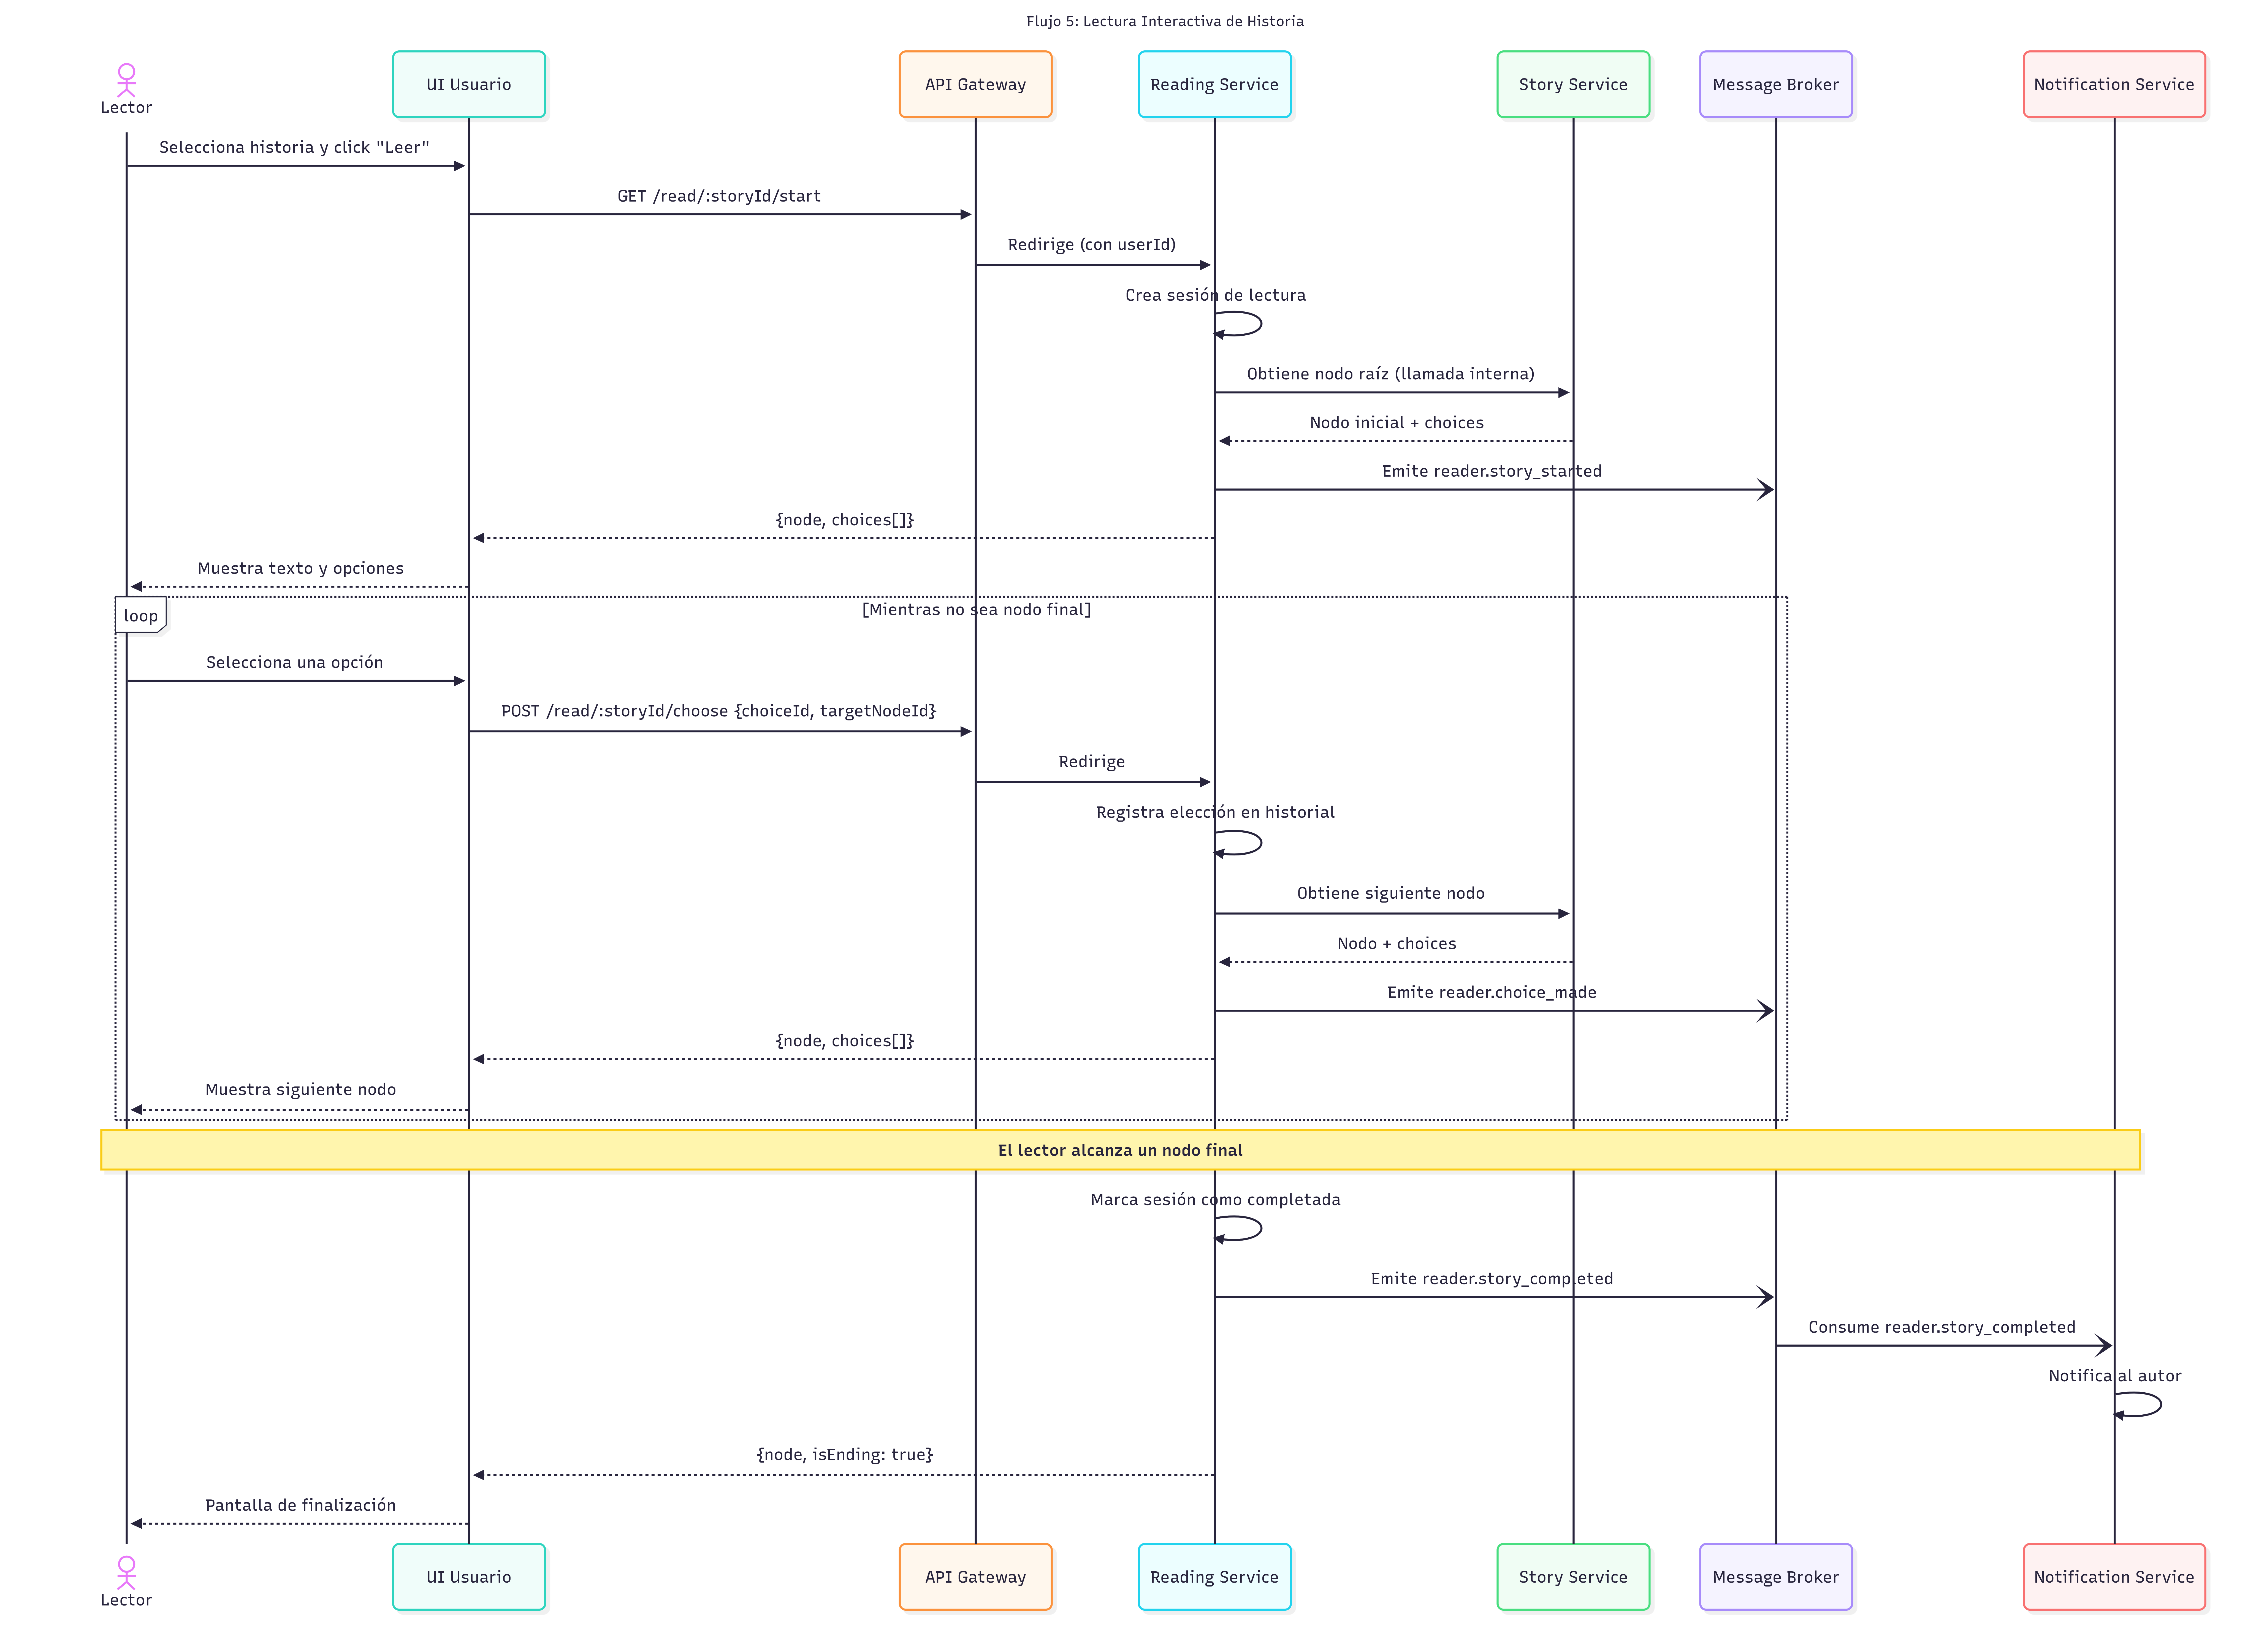
\includegraphics[width=1\textwidth]{images/flujo-read-story.png}
\end{figure}

\subsubsection{Publicación una historia}
El creador solicita publicar su historia. El Story Service ejecuta una validación automática del grafo antes de cambiar el estado de la historia a published. Una vez publicada, emite el evento story.published al servicio de colas. El Notification Service consume este evento de forma asíncrona y notifica a todos los lectores suscritos a ese autor sobre la nueva publicación.
\begin{figure}[H]
    \centering
    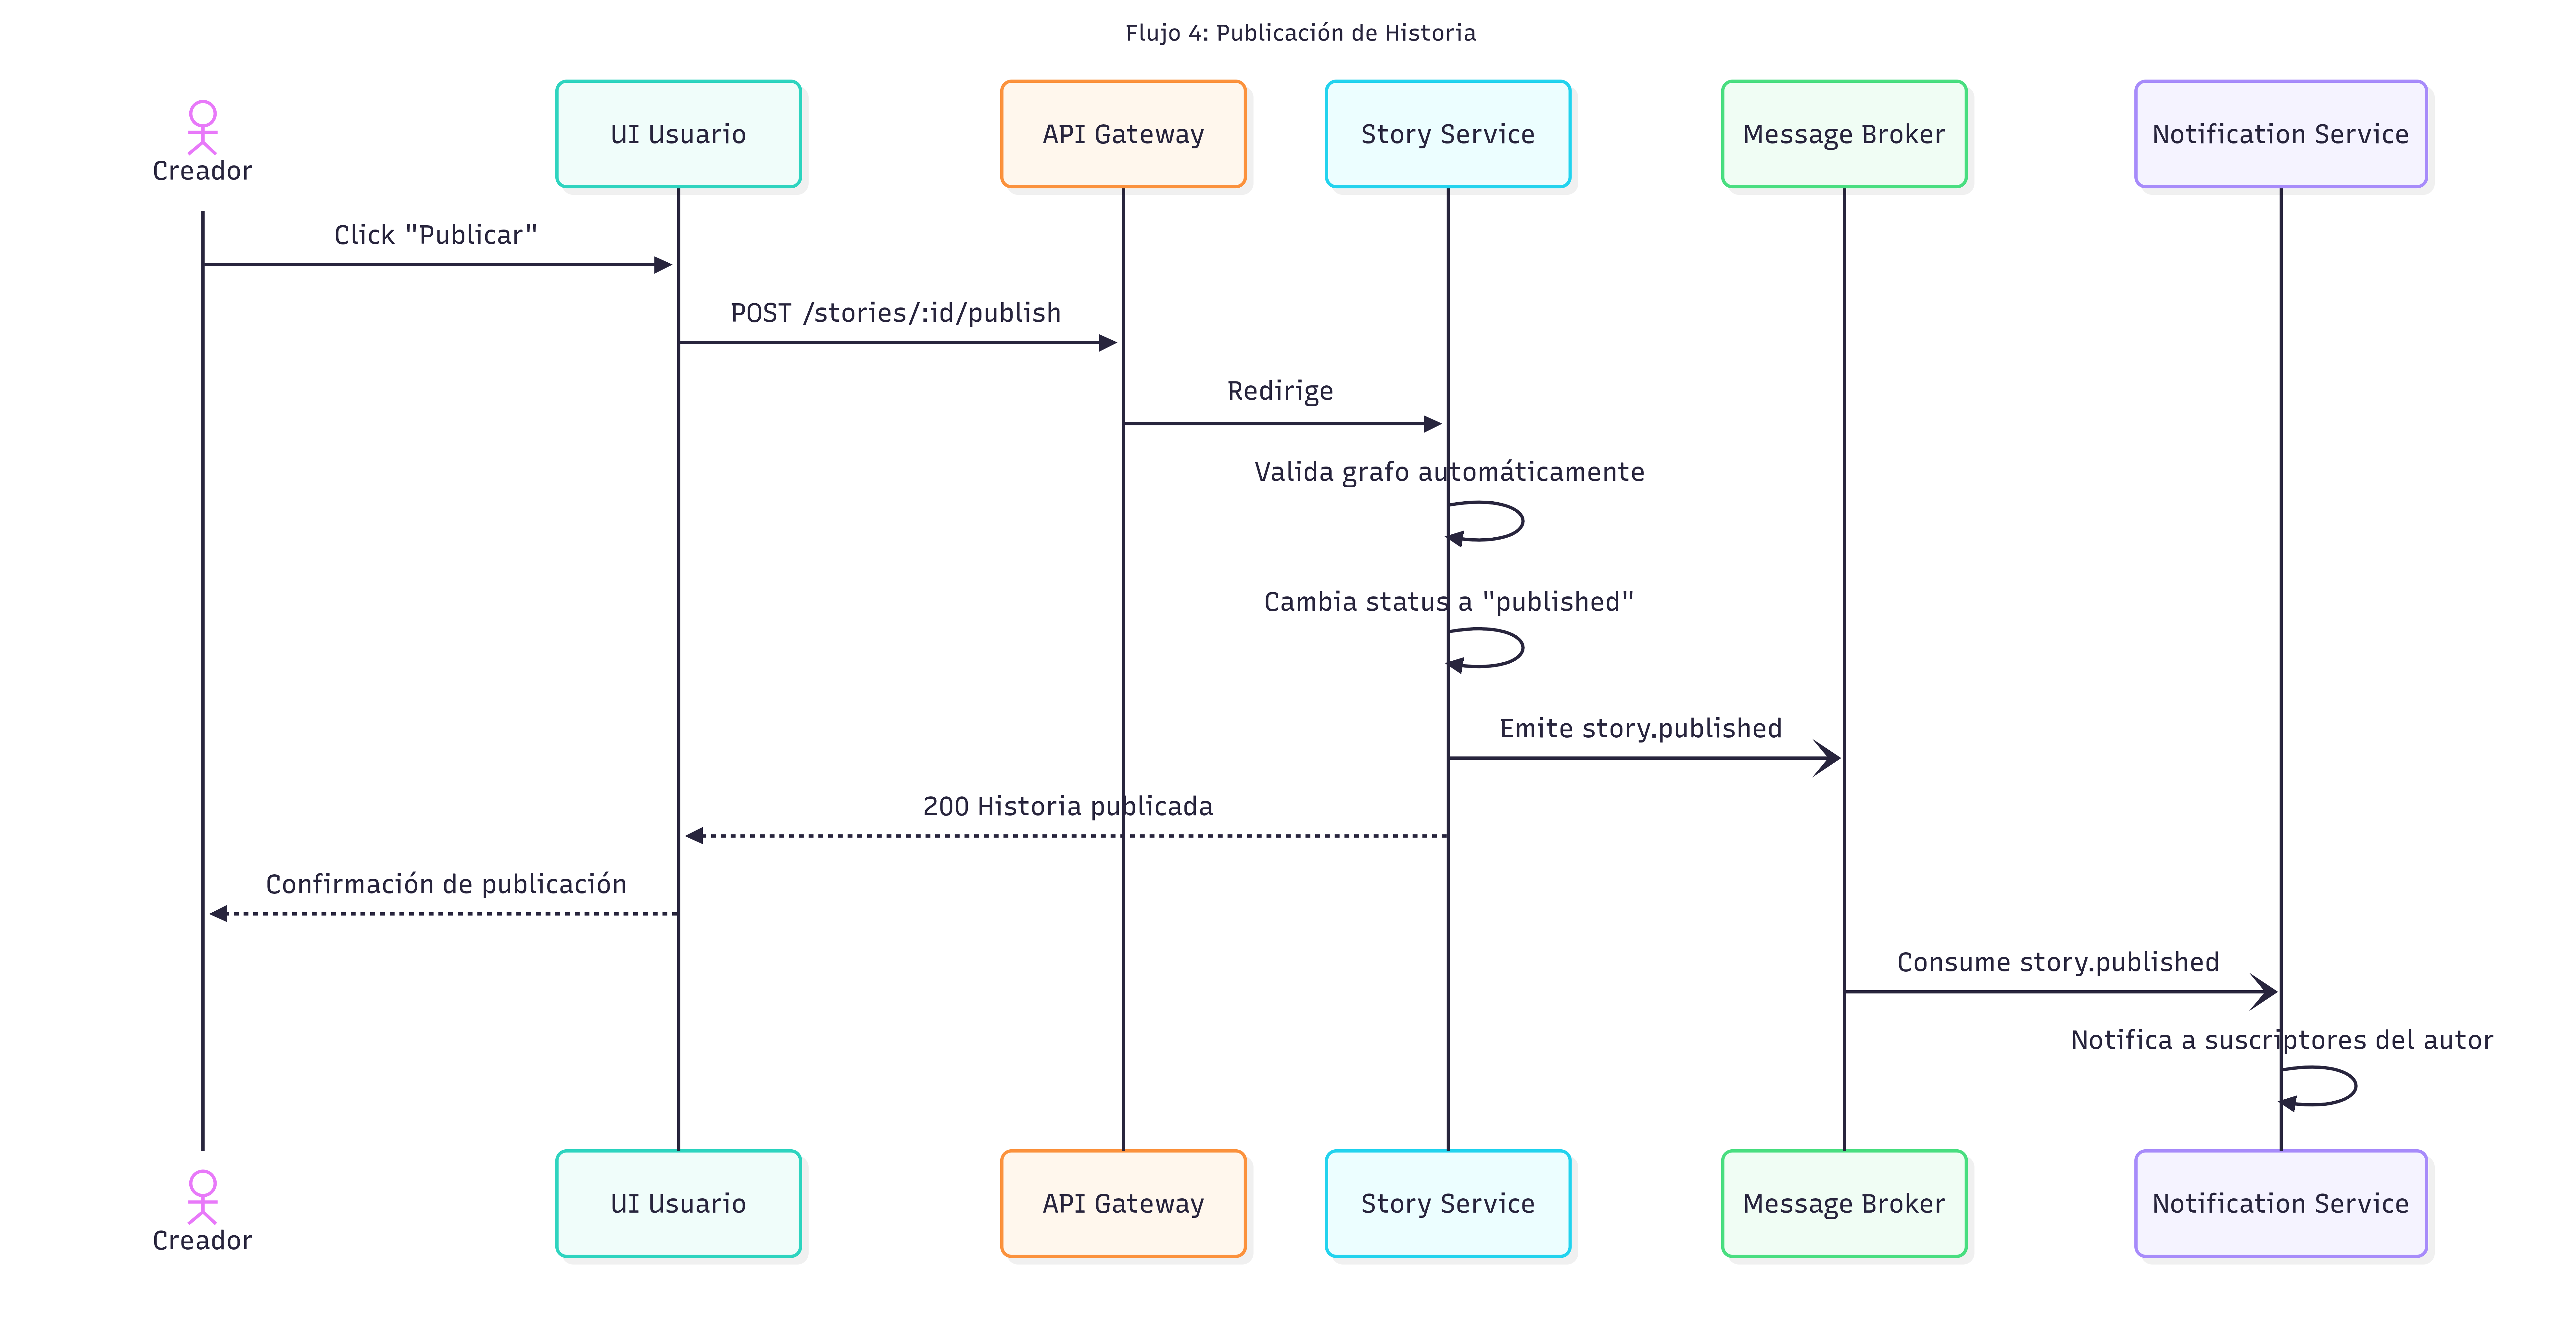
\includegraphics[width=1\textwidth]{images/flujo-publish-story.png}
\end{figure}


\section{Discusión y reflexión}

La estructuración inicial a alto nivel nos proporcionó bases sólidas para la toma de decisiones relacionadas con la selección de tecnologías y servicios, manteniendo una postura deliberadamente agnóstica al proveedor de nube. Este enfoque permitió priorizar capacidades y atributos de calidad sobre herramientas específicas, facilitando la posterior adaptación a un entorno cloud sin comprometer el diseño conceptual del sistema. \\

La arquitectura se abordó mediante una estrategia bottom-up, iniciando desde la capa de persistencia, ya que el dominio del problema está fuertemente centrado en la gestión de nodos y relaciones tipo grafo para soportar historias dinámicas con múltiples caminos narrativos. Este punto de partida permitió alinear tempranamente el modelo de datos con las necesidades funcionales del sistema, reduciendo riesgos de rediseño posterior y favoreciendo la coherencia entre dominio y arquitectura. \\

El proceso de diseño también permitió abstraer las responsabilidades principales del sistema e identificar límites claros entre componentes, promoviendo una descomposición en servicios especializados. Esta decisión favorece atributos de calidad como escalabilidad independiente, mantenibilidad y resiliencia, al permitir evolucionar componentes de forma aislada y tolerar fallos parciales sin afectar la totalidad del sistema. Asimismo, facilita la adopción de principios cloud-native como desacoplamiento, elasticidad y despliegue independiente. \\

El proceso de diseño a alto nivel también nos proporcionó criterio para poder delimitar la idea inicial, permitiendo filtrar decisiones excesivamente ambiciosas que no aportaban valor directo al objetivo del sistema. Esta abstracción temprana ayudó a enfocar el alcance en los componentes esenciales evitando sobreingeniería.


\end{document}